\section{Signal/background comparisons}
\label{app:SignalBackgroundComparison}

\subsection{BDT input variables}
\label{subapp:SOVERB_BDTInputVars}
Figures \ref{fig:SOVERB_HT_jets} to Fig.\ref{fig:SOVERB_tb_ptAsymm} compare the shape of the variables included in the BDT for all $H^{+}$ signal masses and background.

\begin{figure}[H]
  \subfloat[HT\_jets] {
    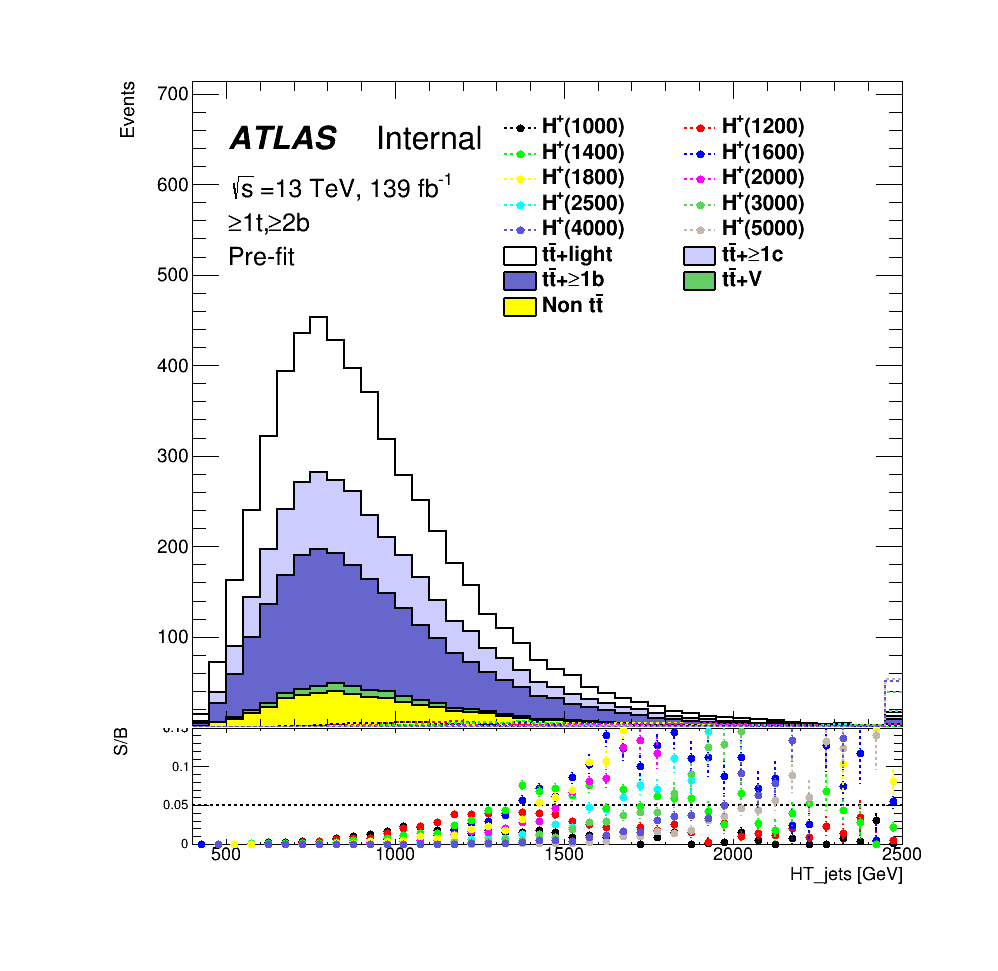
\includegraphics[width=0.25\textwidth]{images/SigBkgComparison/SOVERB_HT_jets_geq1tgeq2b.png}
    \label{fig:SOVERB_HT_jets}
  }
  \subfloat[LeadingJet\_pt] {
    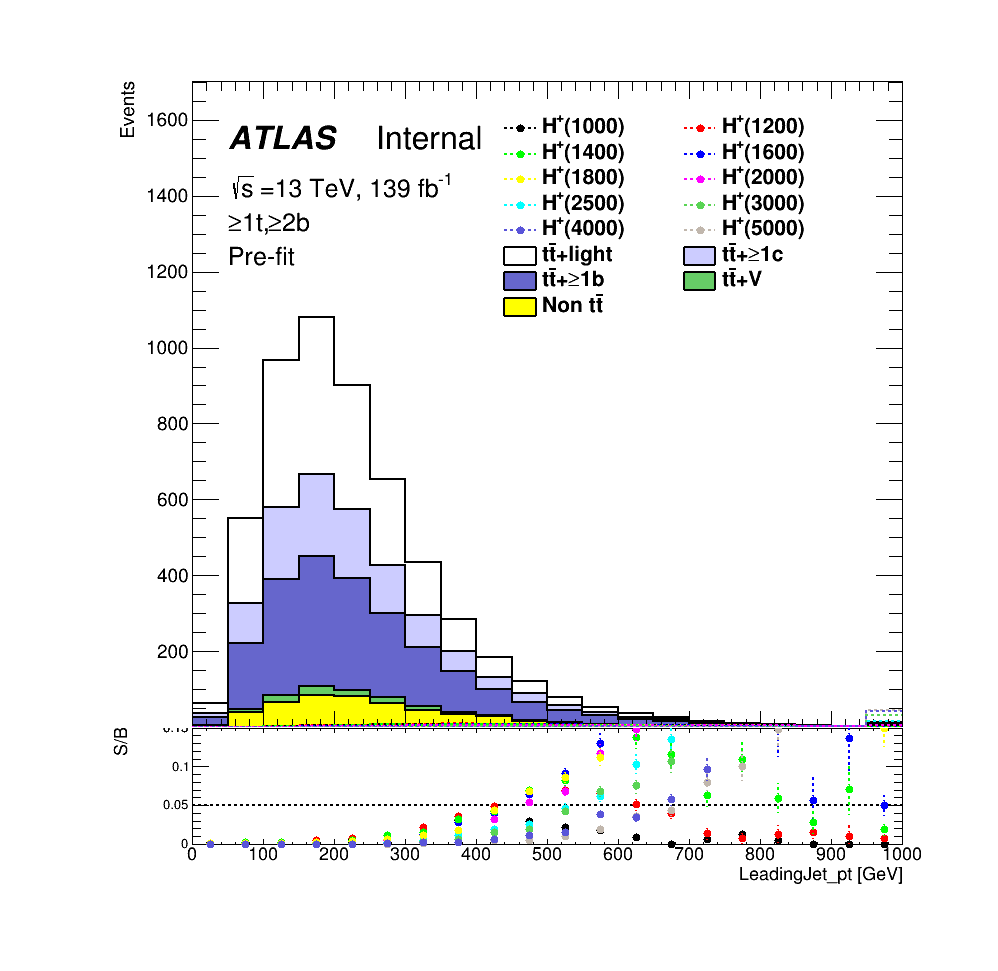
\includegraphics[width=0.25\textwidth]{images/SigBkgComparison/SOVERB_LeadingJet_pt_geq1tgeq2b.png}
    \label{fig:SOVERB_LeadingJet_pt}
  }
  \subfloat[Centrality\_all] {
    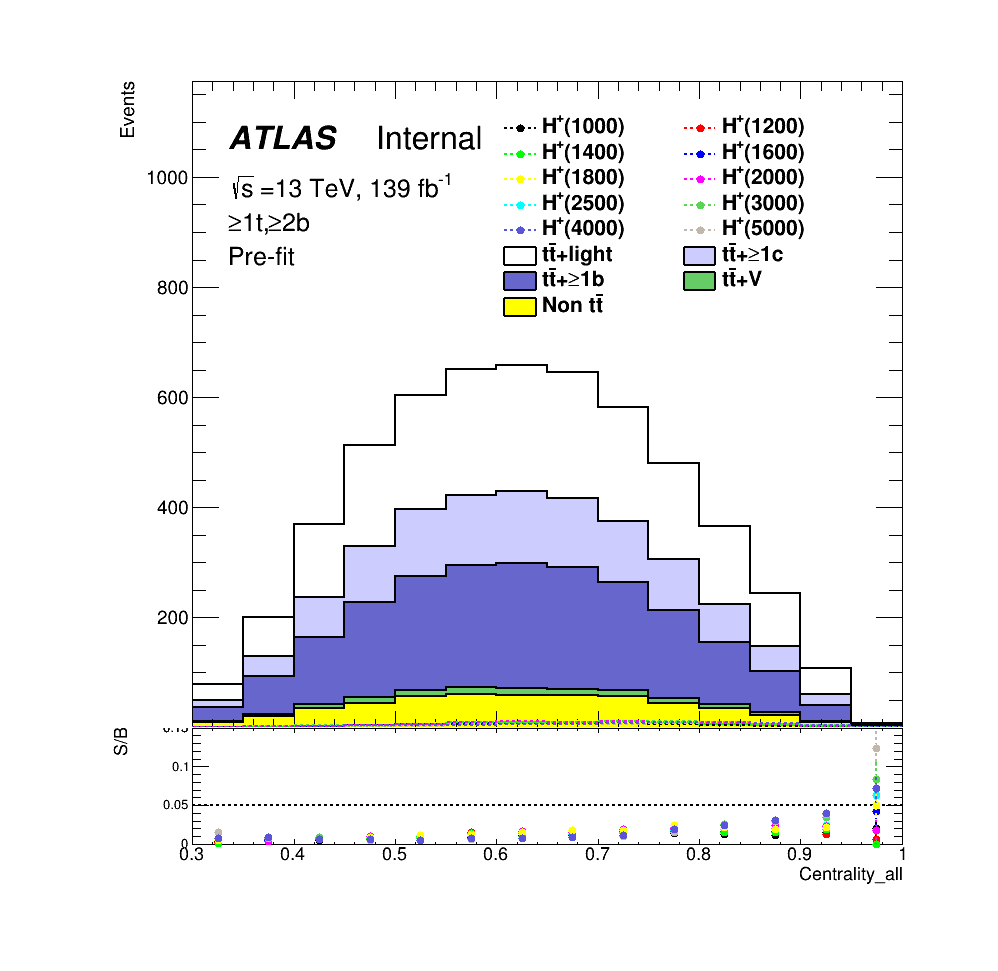
\includegraphics[width=0.25\textwidth]{images/SigBkgComparison/SOVERB_Centrality_all_geq1tgeq2b.png}
    \label{fig:SOVERB_Centrality_all}
  }
  \subfloat[H1\_all] {
    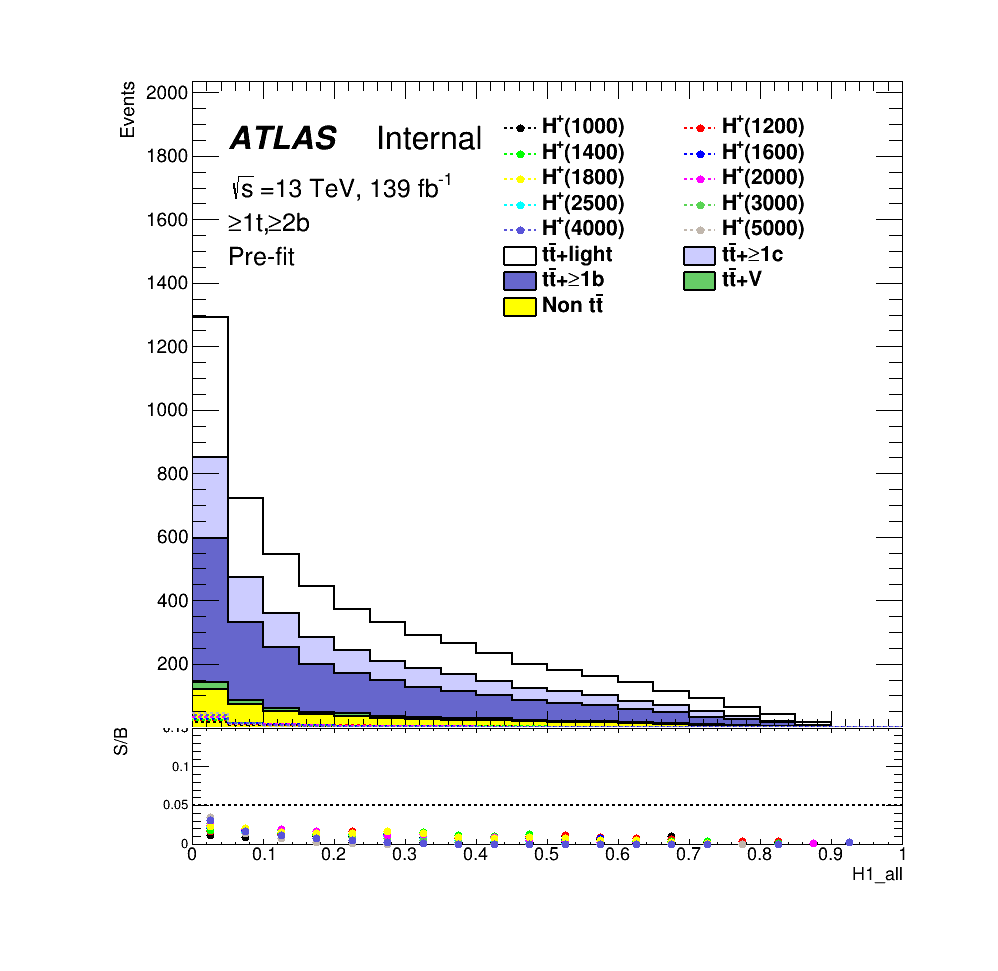
\includegraphics[width=0.25\textwidth]{images/SigBkgComparison/SOVERB_H1_all_geq1tgeq2b.png}
    \label{fig:SOVERB_H1_all}
  }\\
  \subfloat[Mbb\_MaxPt] {
    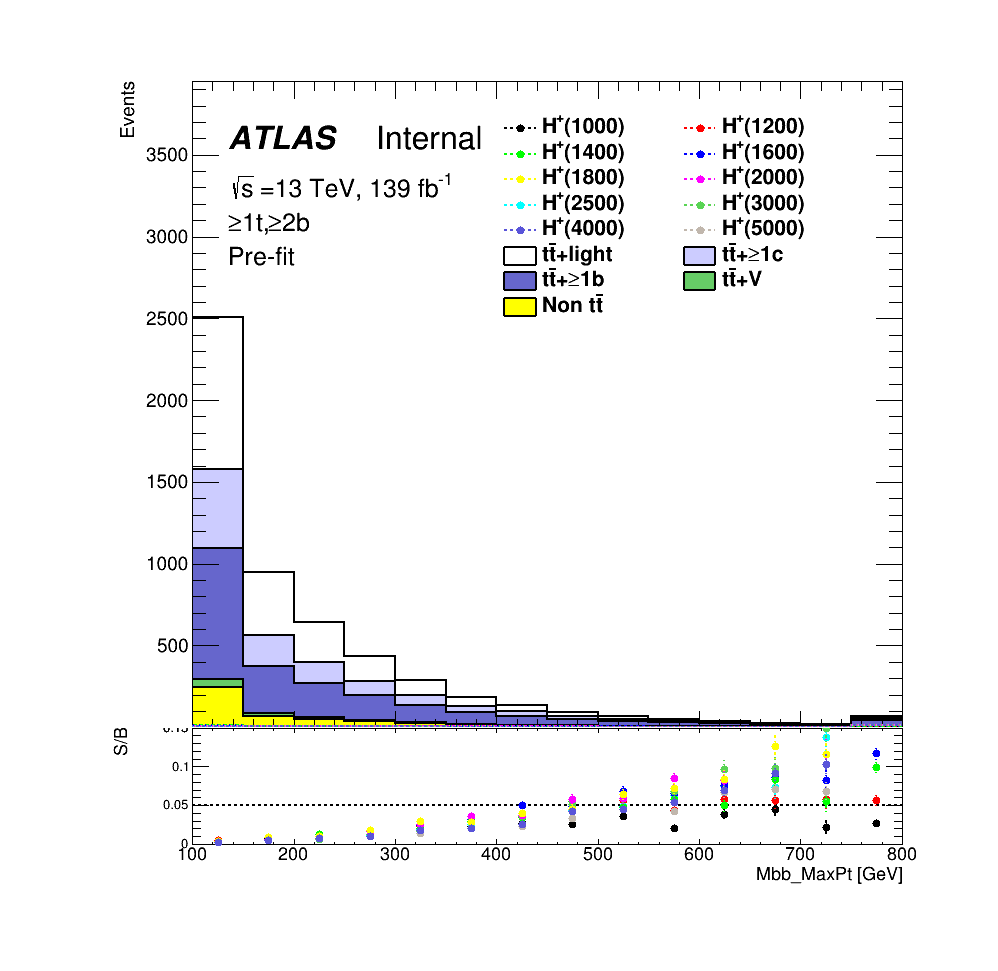
\includegraphics[width=0.25\textwidth]{images/SigBkgComparison/SOVERB_Mbb_MaxPt_geq1tgeq2b.png}
    \label{fig:SOVERB_Mbb_MaxPt}
  }
  \subfloat[Mjjj\_MaxPt] {
    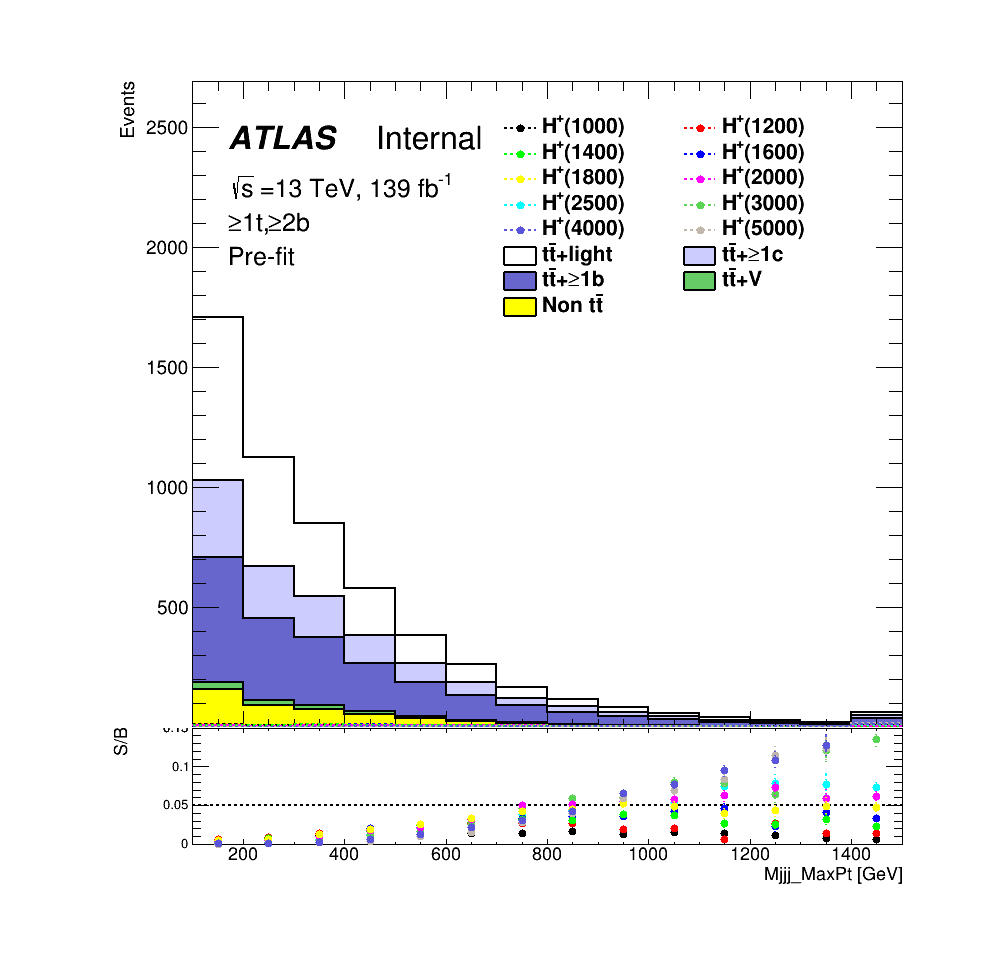
\includegraphics[width=0.25\textwidth]{images/SigBkgComparison/SOVERB_Mjjj_MaxPt_geq1tgeq2b.png}
    \label{fig:SOVERB_Mjjj_MaxPt}
  }
  \subfloat[Muu\_MindR] {
    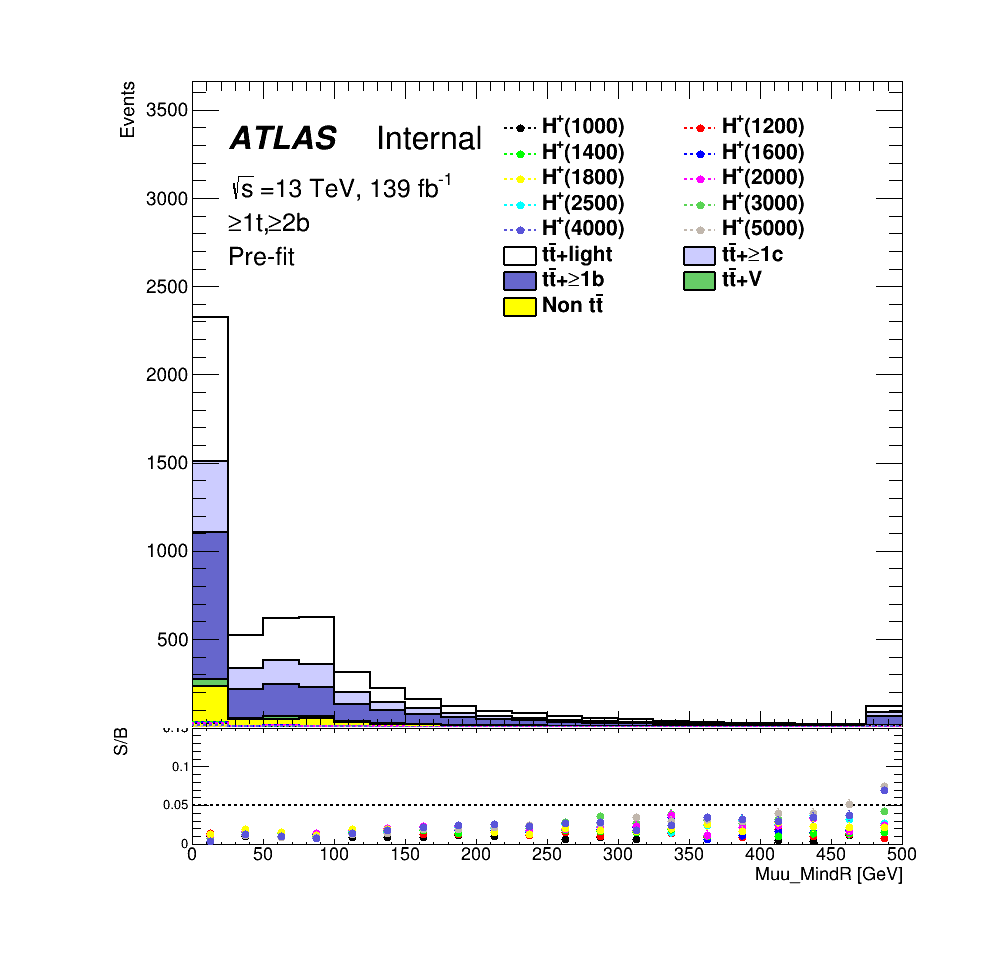
\includegraphics[width=0.25\textwidth]{images/SigBkgComparison/SOVERB_Muu_MindR_geq1tgeq2b.png}
    \label{fig:SOVERB_Muu_MindR}
  }
  \subfloat[dRbb\_avg] {
    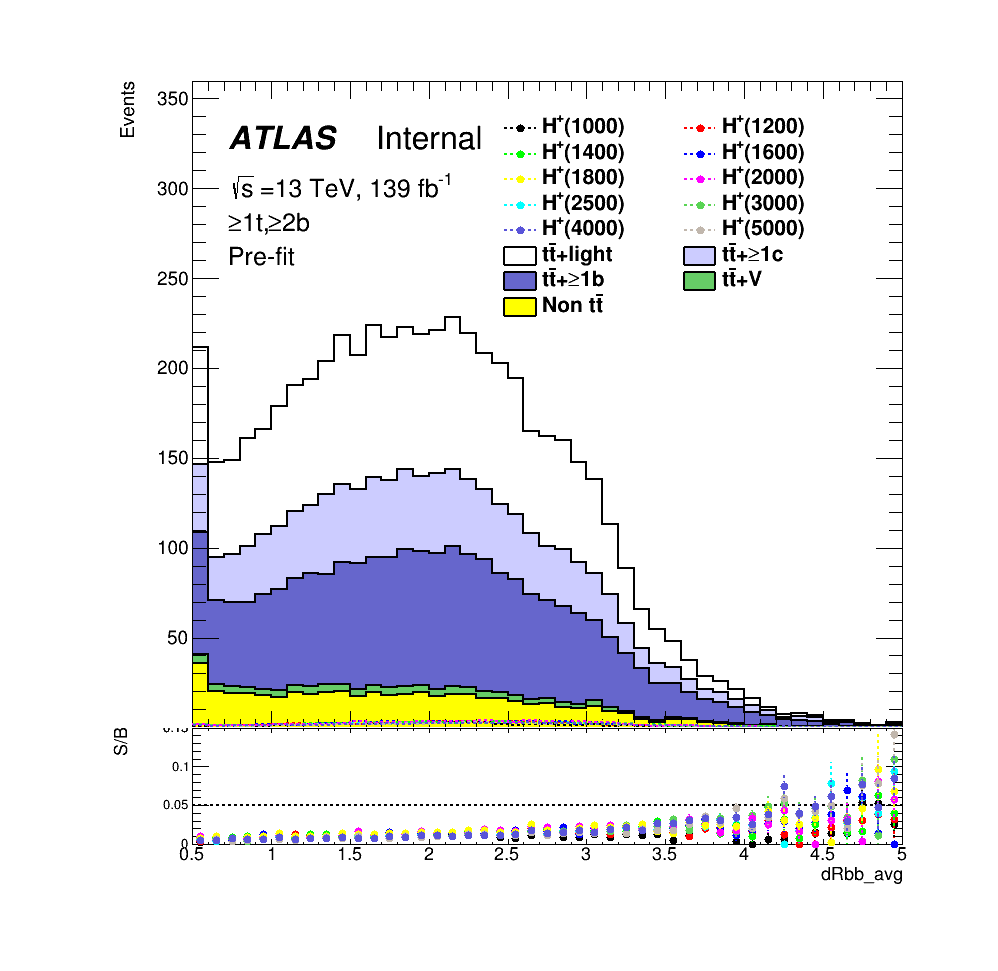
\includegraphics[width=0.25\textwidth]{images/SigBkgComparison/SOVERB_dRbb_avg_geq1tgeq2b.png}
    \label{fig:SOVERB_dRbb_avg}
  }\\
  \subfloat[dRlepbb\_MindR] {
    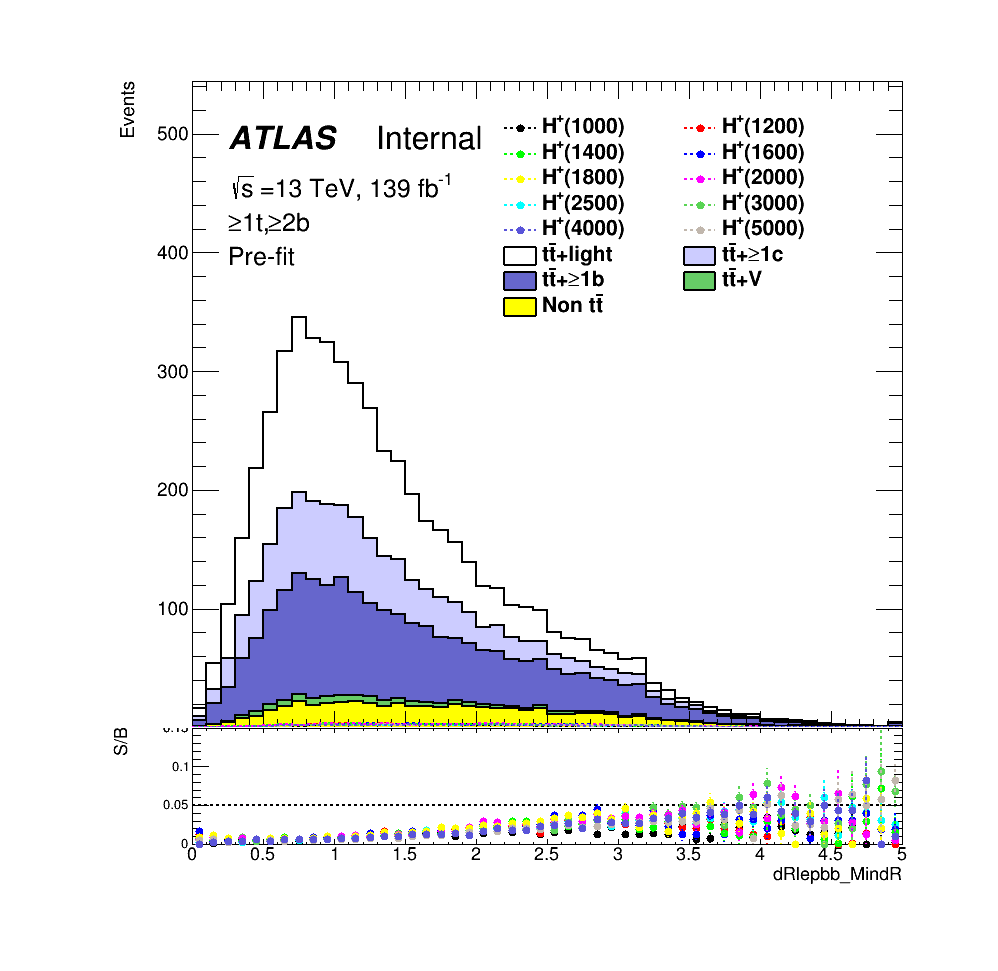
\includegraphics[width=0.25\textwidth]{images/SigBkgComparison/SOVERB_dRlepbb_MindR_geq1tgeq2b.png}
    \label{fig:SOVERB_dRlepbb_MindR}
  }
  \subfloat[LeadingTop\_m] {
    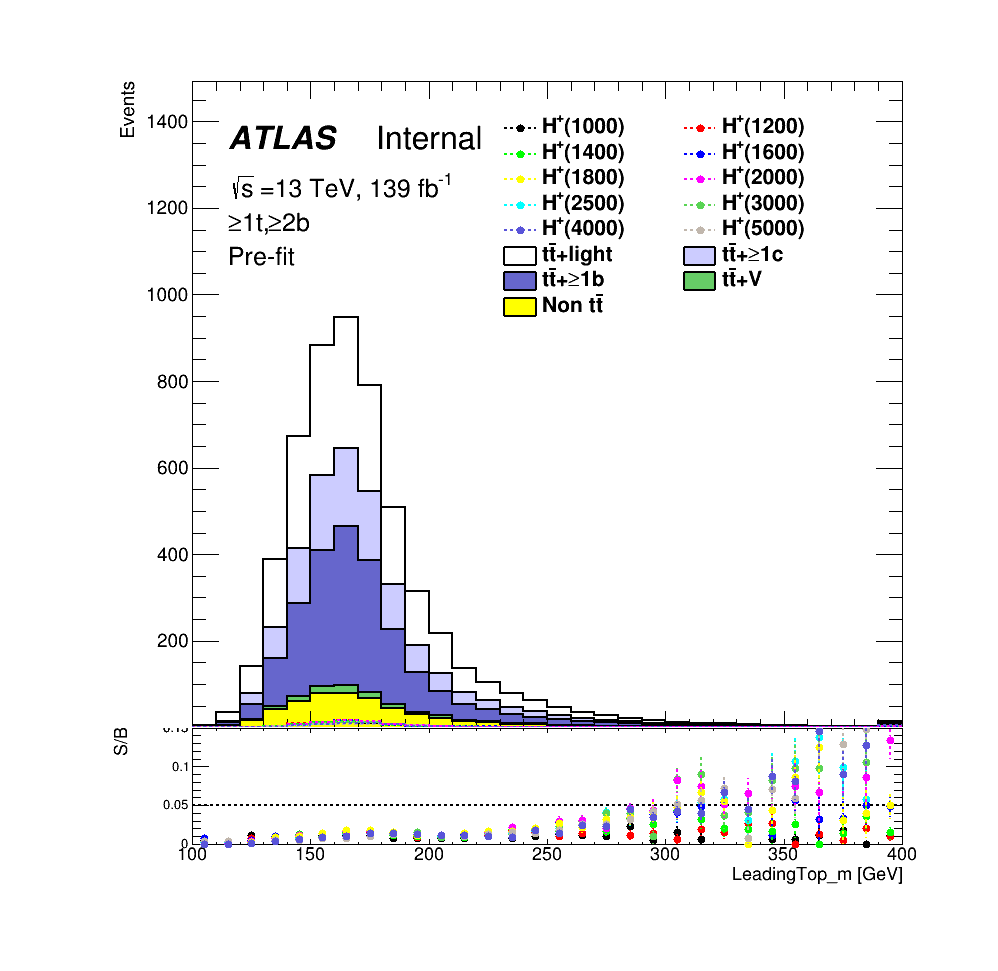
\includegraphics[width=0.25\textwidth]{images/SigBkgComparison/SOVERB_LeadingTop_mass_geq1tgeq2b.png}
    \label{fig:SOVERB_LeadingTop_mass}
  }
  \subfloat[LeadingTop\_pt] {
    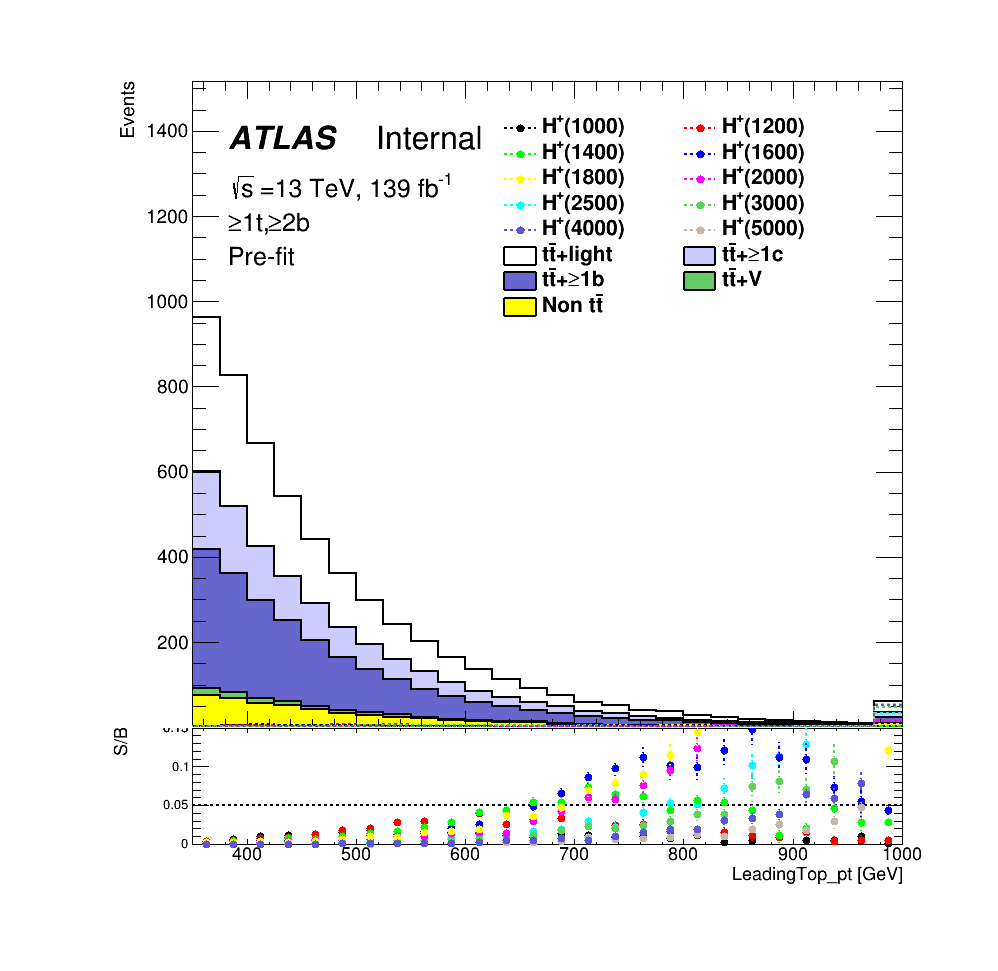
\includegraphics[width=0.25\textwidth]{images/SigBkgComparison/SOVERB_LeadingTop_pt_geq1tgeq2b.png}
    \label{fig:SOVERB_LeadingTop_pt}
  }
  \subfloat[M\_tb] {
    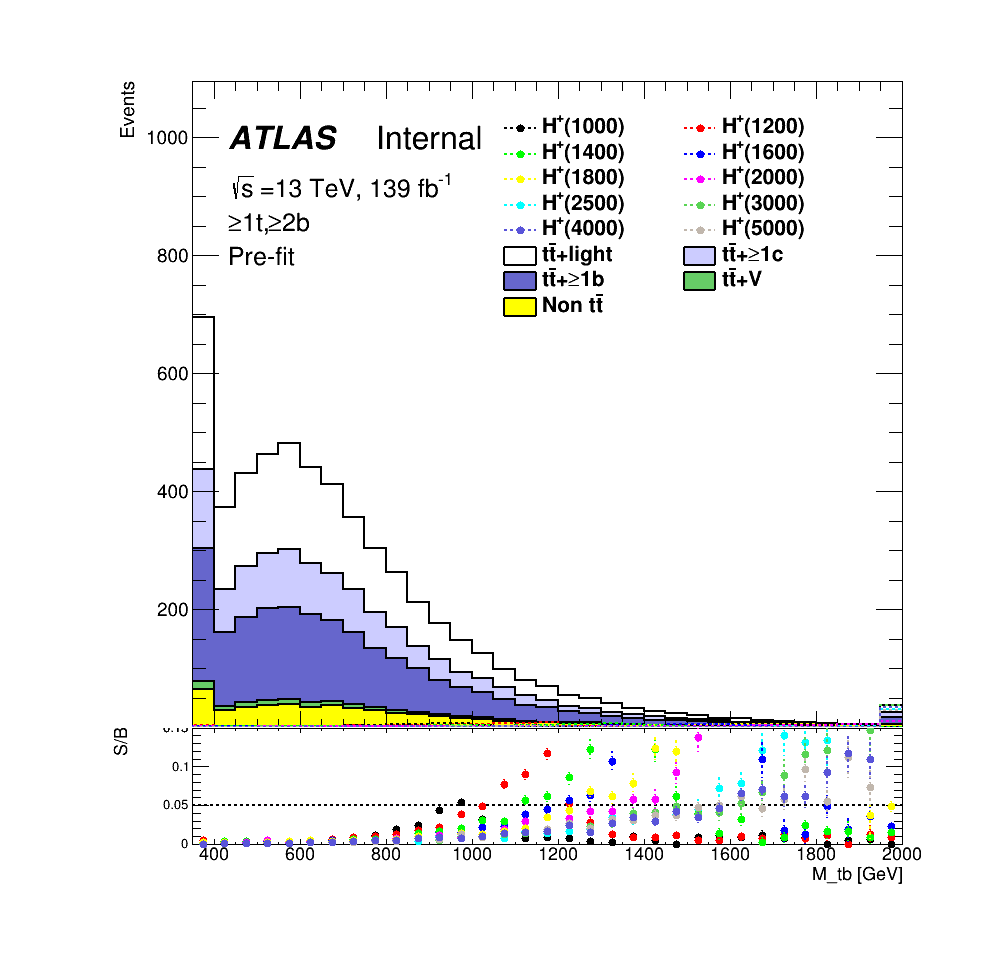
\includegraphics[width=0.25\textwidth]{images/SigBkgComparison/SOVERB_tb_mass_geq1tgeq2b.png}
    \label{fig:SOVERB_tb_mass}
  }\\
  \subfloat[Pt\_tb] {
    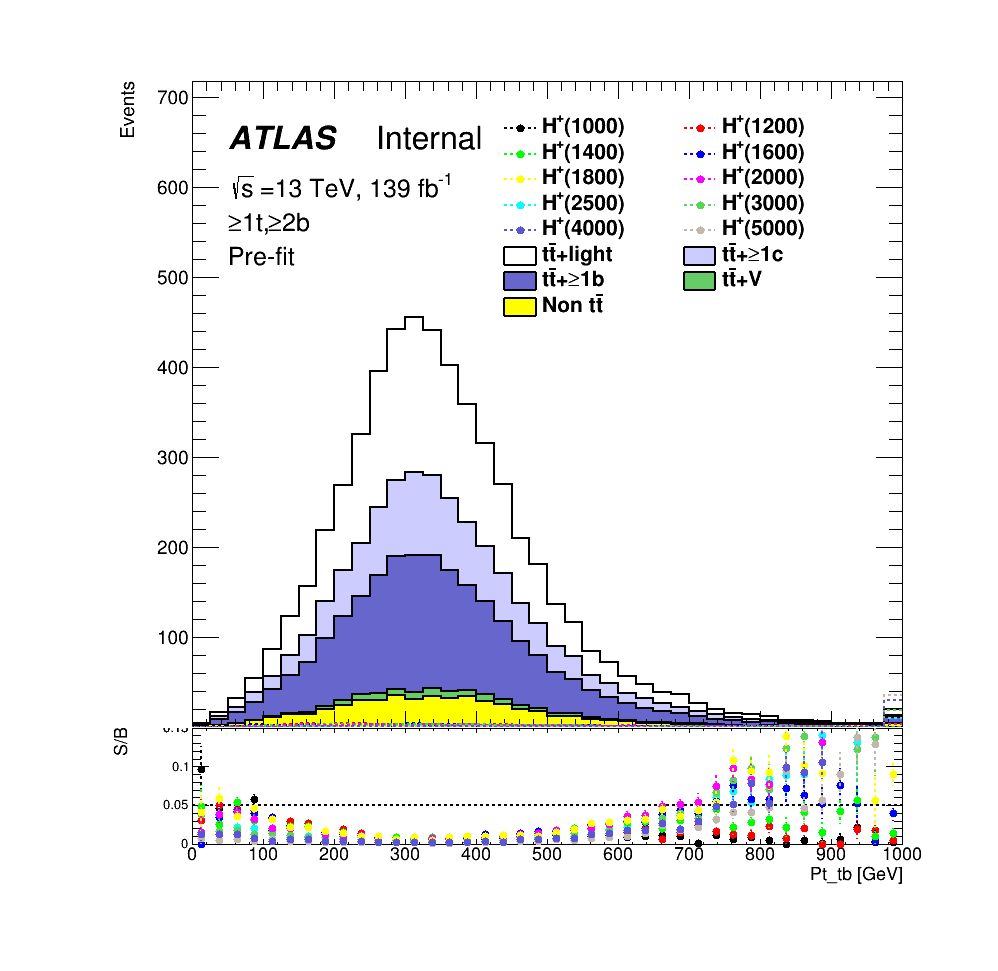
\includegraphics[width=0.25\textwidth]{images/SigBkgComparison/SOVERB_tb_pt_geq1tgeq2b.png}
    \label{fig:SOVERB_tb_pt}
  }
  \subfloat[PtAsymm\_tb] {
    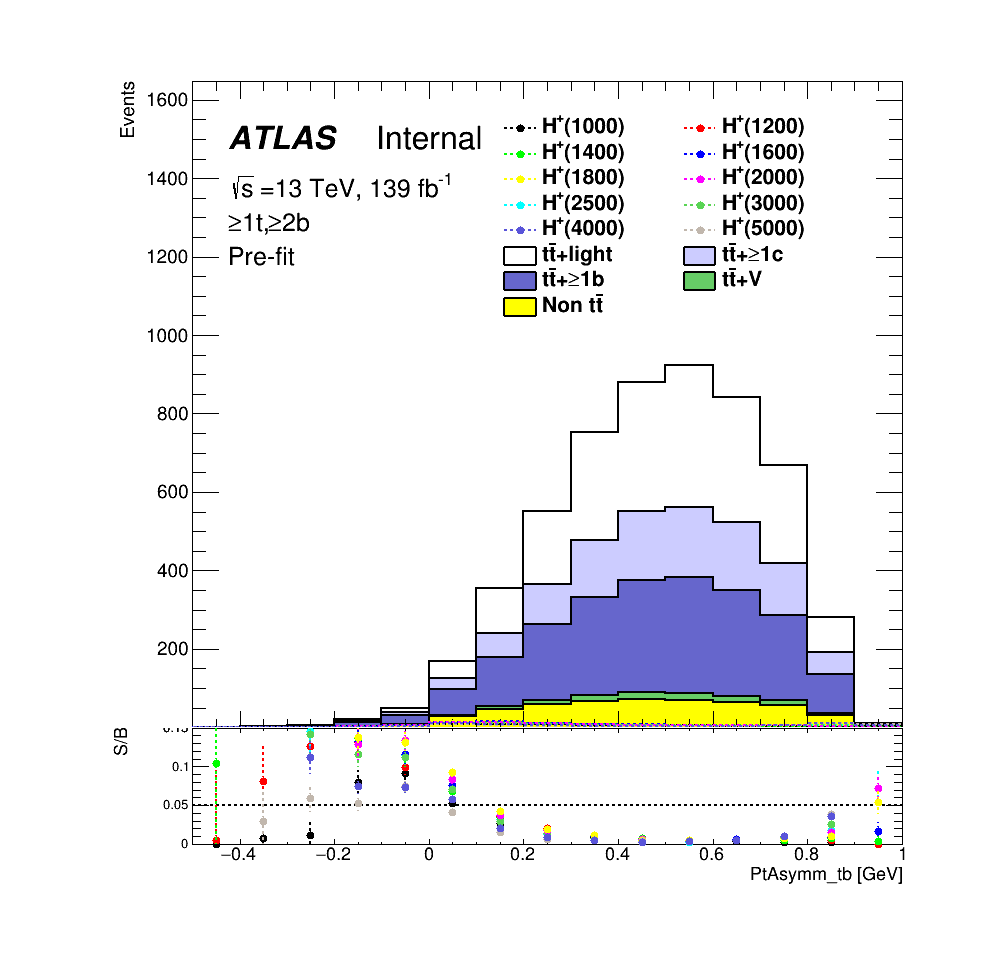
\includegraphics[width=0.25\textwidth]{images/SigBkgComparison/SOVERB_tb_ptAsymm_geq1tgeq2b.png}
    \label{fig:SOVERB_tb_ptAsymm}
  }
  \caption{Comparison of the kinematic variables included in the BDT in the SR for the various $H^{+}$ signal masses between signal and background.}
  \label{fig:SOVERB_BDTInputs}
\end{figure}
\subsection{BDT output}
\label{subapp:SOVERB_BDTOutput}
Figures \ref{fig:SOVERB_bdt_Hp1000_equivBinning_geq1tgeq2b} to Fig.\ref{fig:SOVERB_bdt_Hp5000_equivBinning_geq1tgeq2b} compare the shape of BDT output distribution in SR region between the signal and background on each  $H^{+}$ signal mass hypothesis at equal bin intervals.

\begin{figure}[H]
  \subfloat[] {
    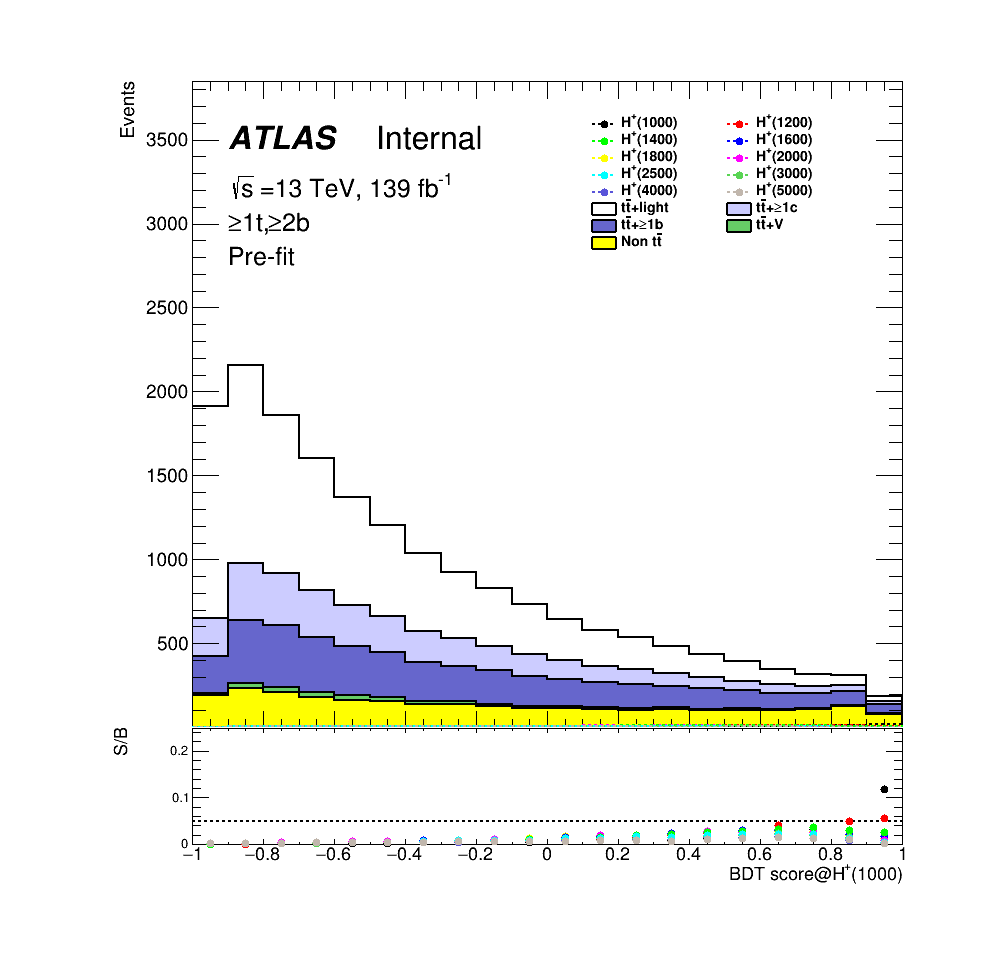
\includegraphics[width=0.30\textwidth]{images/SigBkgComparison/SOVERB_bdt_Hp1000_equivBinning_geq1tgeq2b.png}
    \label{fig:SOVERB_bdt_Hp1000_equivBinning_geq1tgeq2b}
  }
  \subfloat[] {
    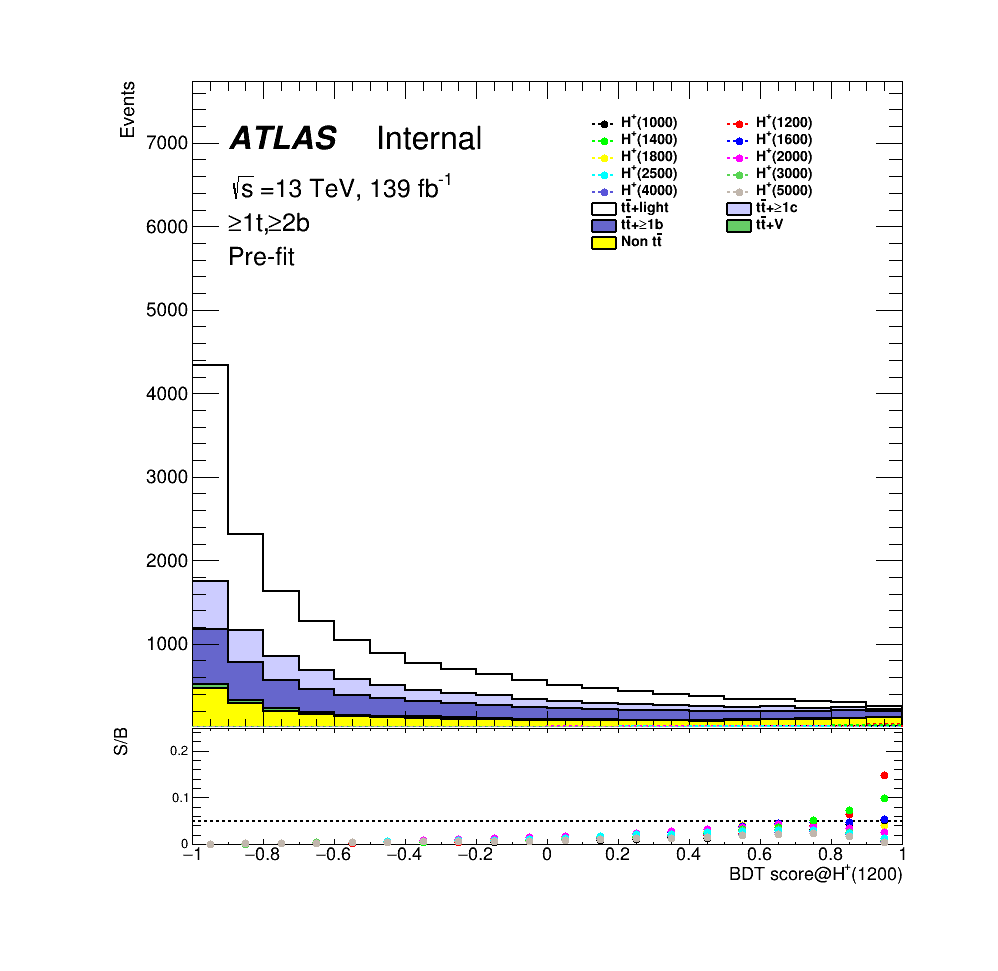
\includegraphics[width=0.30\textwidth]{images/SigBkgComparison/SOVERB_bdt_Hp1200_equivBinning_geq1tgeq2b.png}
    \label{fig:SOVERB_bdt_Hp1200_equivBinning_geq1tgeq2b}
  }
  \subfloat[] {
    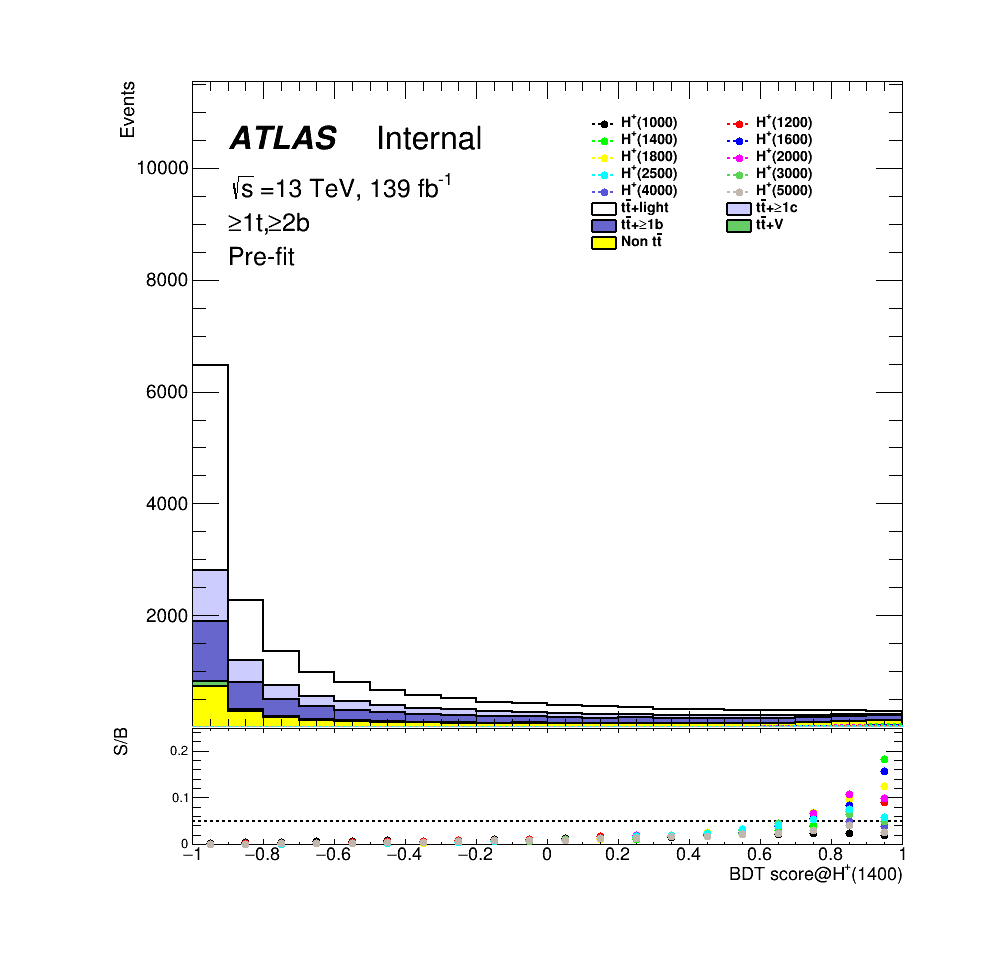
\includegraphics[width=0.30\textwidth]{images/SigBkgComparison/SOVERB_bdt_Hp1400_equivBinning_geq1tgeq2b.png}
    \label{fig:SOVERB_bdt_Hp1400_equivBinning_geq1tgeq2b}
  }\\
  \subfloat[] {
    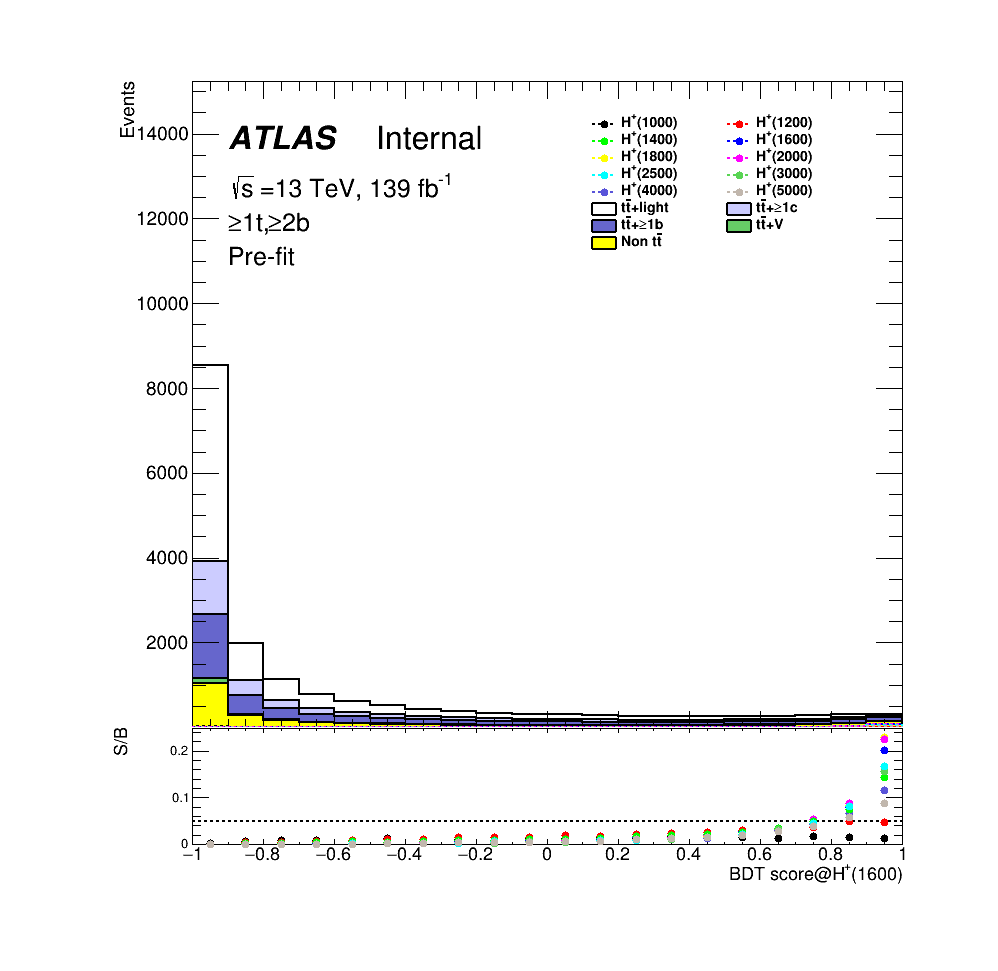
\includegraphics[width=0.30\textwidth]{images/SigBkgComparison/SOVERB_bdt_Hp1600_equivBinning_geq1tgeq2b.png}
    \label{fig:SOVERB_bdt_Hp1600_equivBinning_geq1tgeq2b}
  }
  \subfloat[] {
    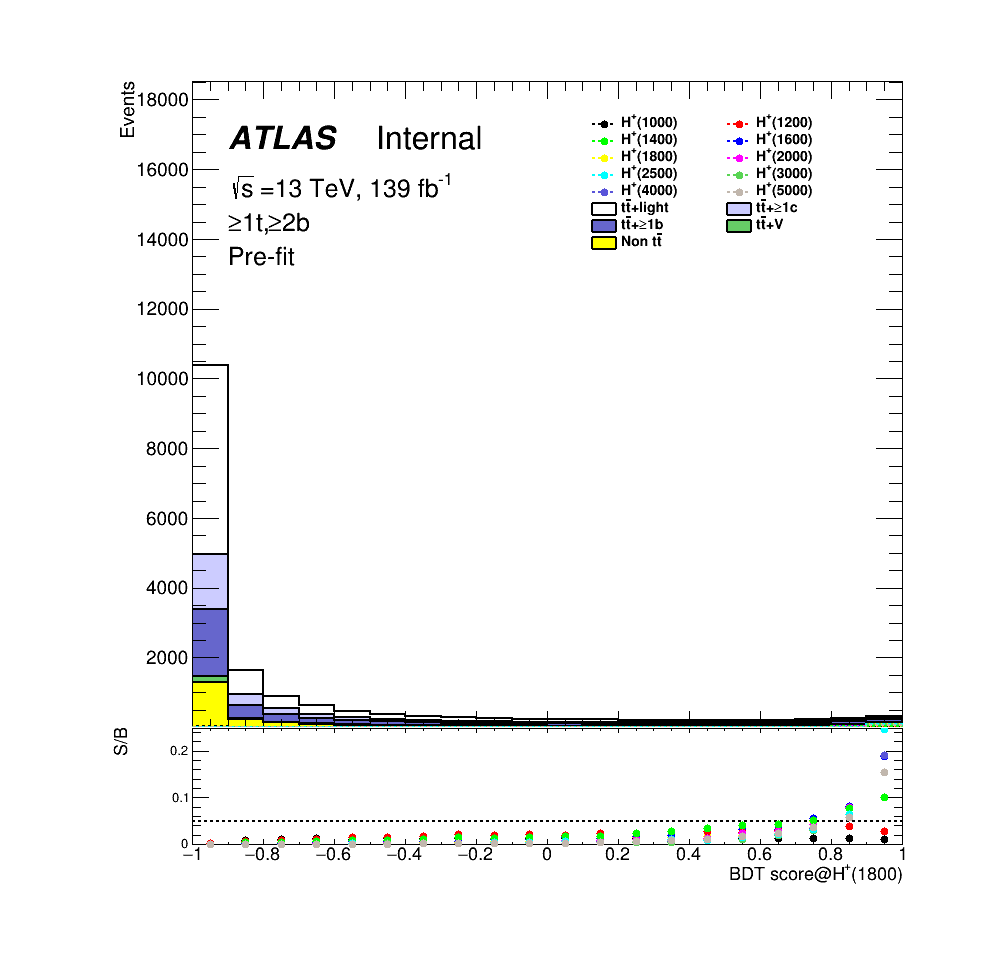
\includegraphics[width=0.30\textwidth]{images/SigBkgComparison/SOVERB_bdt_Hp1800_equivBinning_geq1tgeq2b.png}
    \label{fig:SOVERB_bdt_Hp1800_equivBinning_geq1tgeq2b}
  }
  \subfloat[] {
    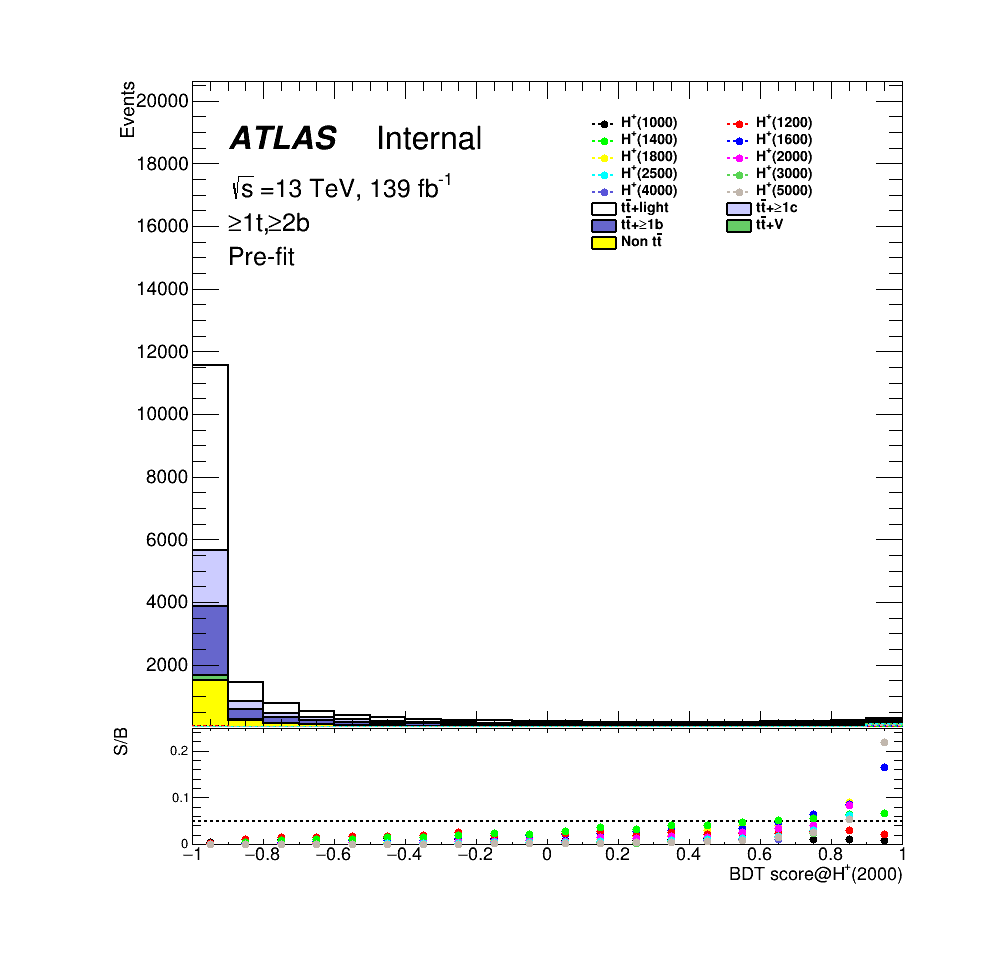
\includegraphics[width=0.30\textwidth]{images/SigBkgComparison/SOVERB_bdt_Hp2000_equivBinning_geq1tgeq2b.png}
    \label{fig:SOVERB_bdt_Hp2000_equivBinning_geq1tgeq2b}
  }\\
  \subfloat[] {
    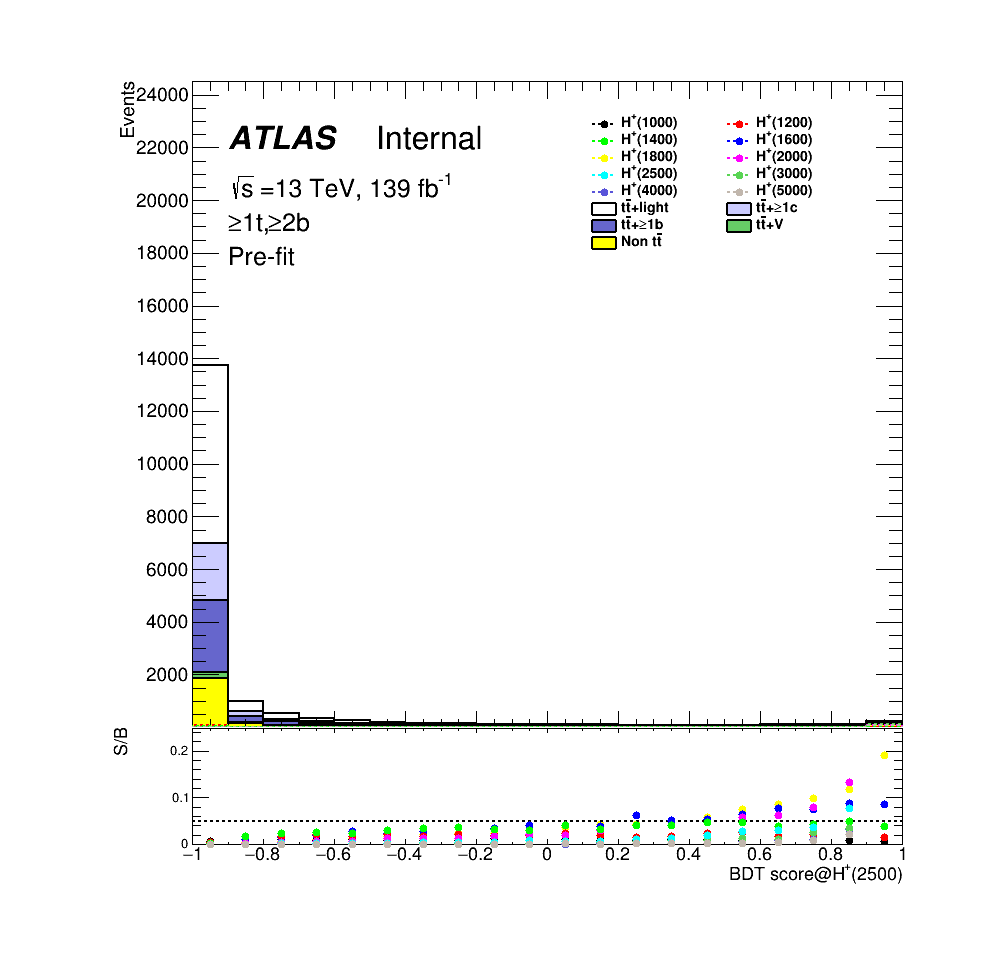
\includegraphics[width=0.30\textwidth]{images/SigBkgComparison/SOVERB_bdt_Hp2500_equivBinning_geq1tgeq2b.png}
    \label{fig:SOVERB_bdt_Hp2500_equivBinning_geq1tgeq2b}
  }
  \subfloat[] {
    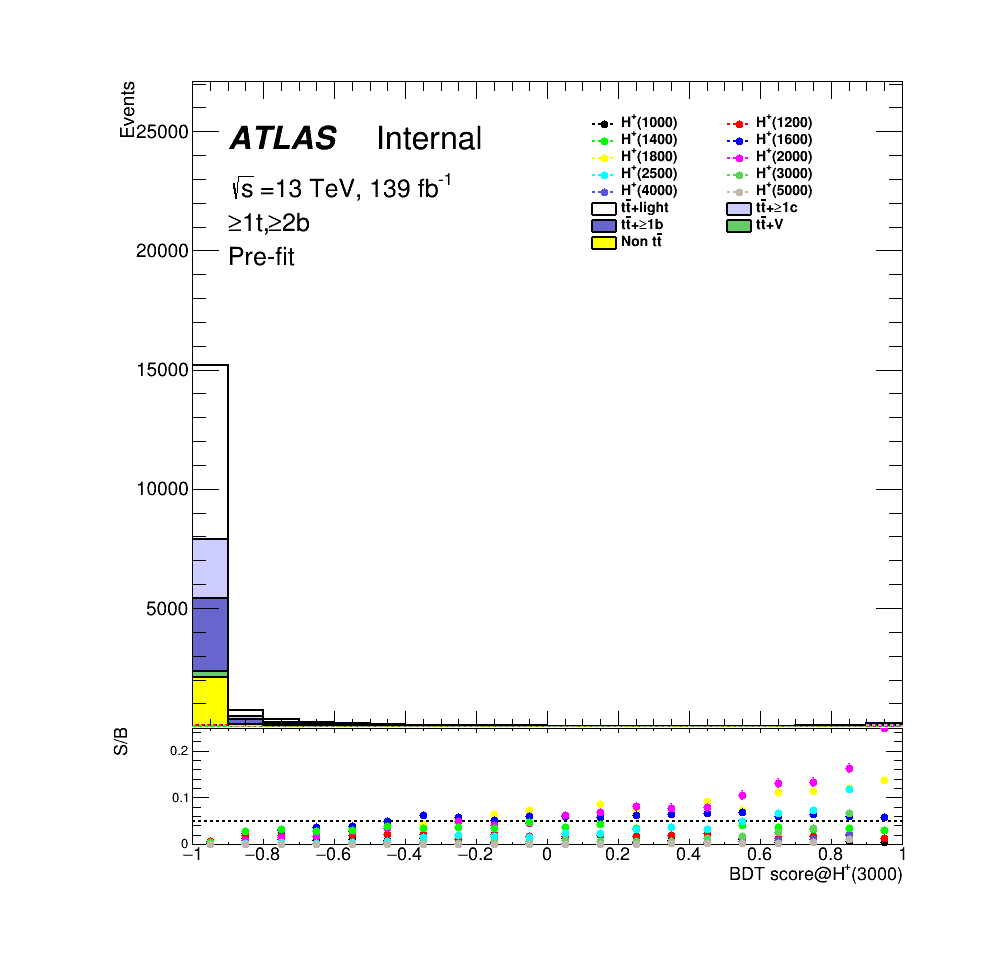
\includegraphics[width=0.30\textwidth]{images/SigBkgComparison/SOVERB_bdt_Hp3000_equivBinning_geq1tgeq2b.png}
    \label{fig:SOVERB_bdt_Hp3000_equivBinning_geq1tgeq2b}
  }
  \subfloat[] {
    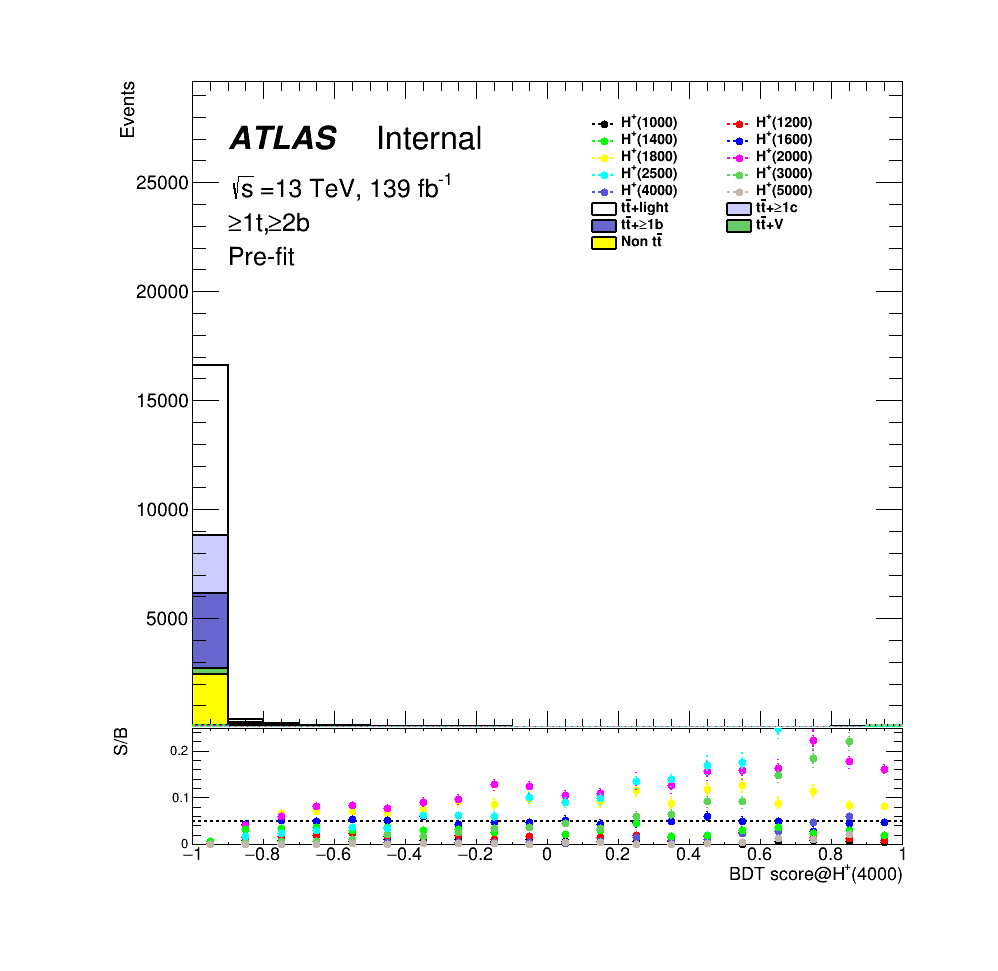
\includegraphics[width=0.30\textwidth]{images/SigBkgComparison/SOVERB_bdt_Hp4000_equivBinning_geq1tgeq2b.png}
    \label{fig:SOVERB_bdt_Hp4000_equivBinning_geq1tgeq2b}
  }\\
  \subfloat[] {
    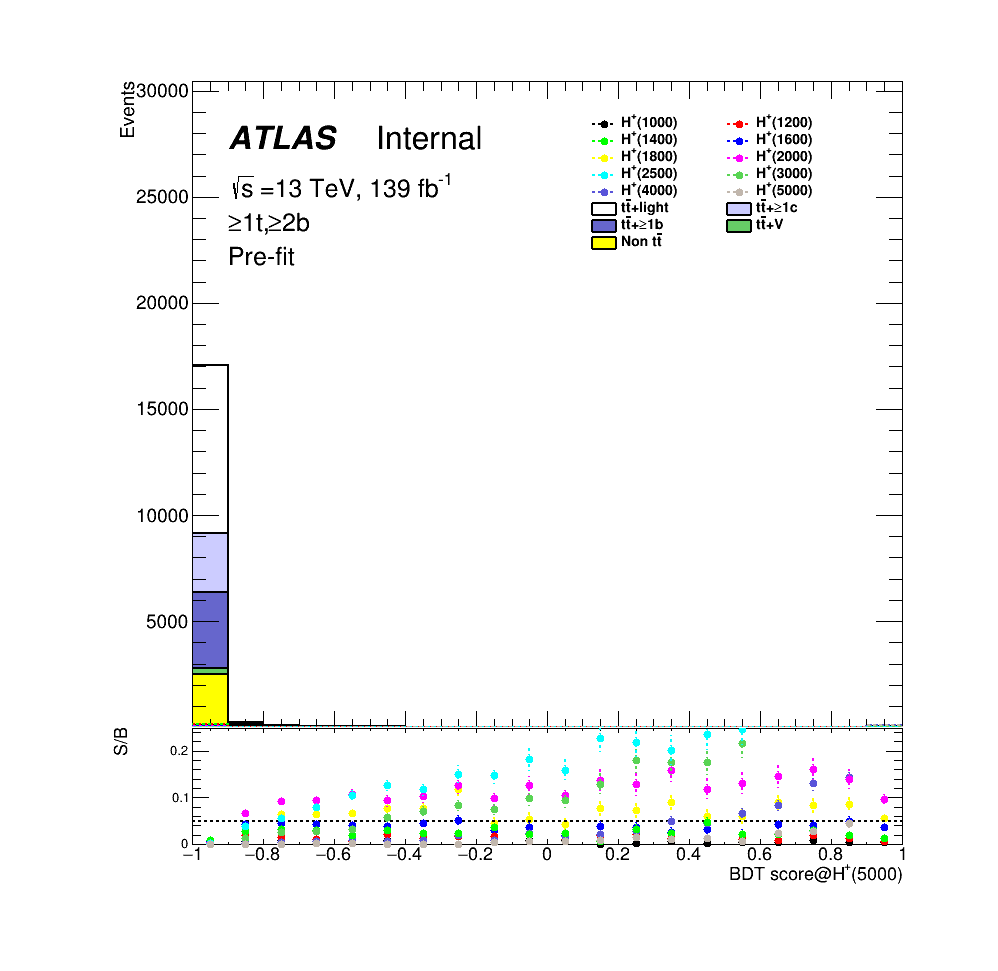
\includegraphics[width=0.30\textwidth]{images/SigBkgComparison/SOVERB_bdt_Hp5000_equivBinning_geq1tgeq2b.png}
    \label{fig:SOVERB_bdt_Hp5000_equivBinning_geq1tgeq2b}
  }
\end{figure}  

Figures \ref{fig:SOVERB_bdt_Hp1000_geq1tgeq2b} to Fig.\ref{fig:SOVERB_bdt_Hp5000_geq1tgeq2b} compare the shape of BDT output distribution in SR region between the signal and background on each  $H^{+}$ signal mass hypothesis at not equal bin intervals. These binning is optimised using TRExFitter.

\begin{figure}[H]
  \subfloat[] {
    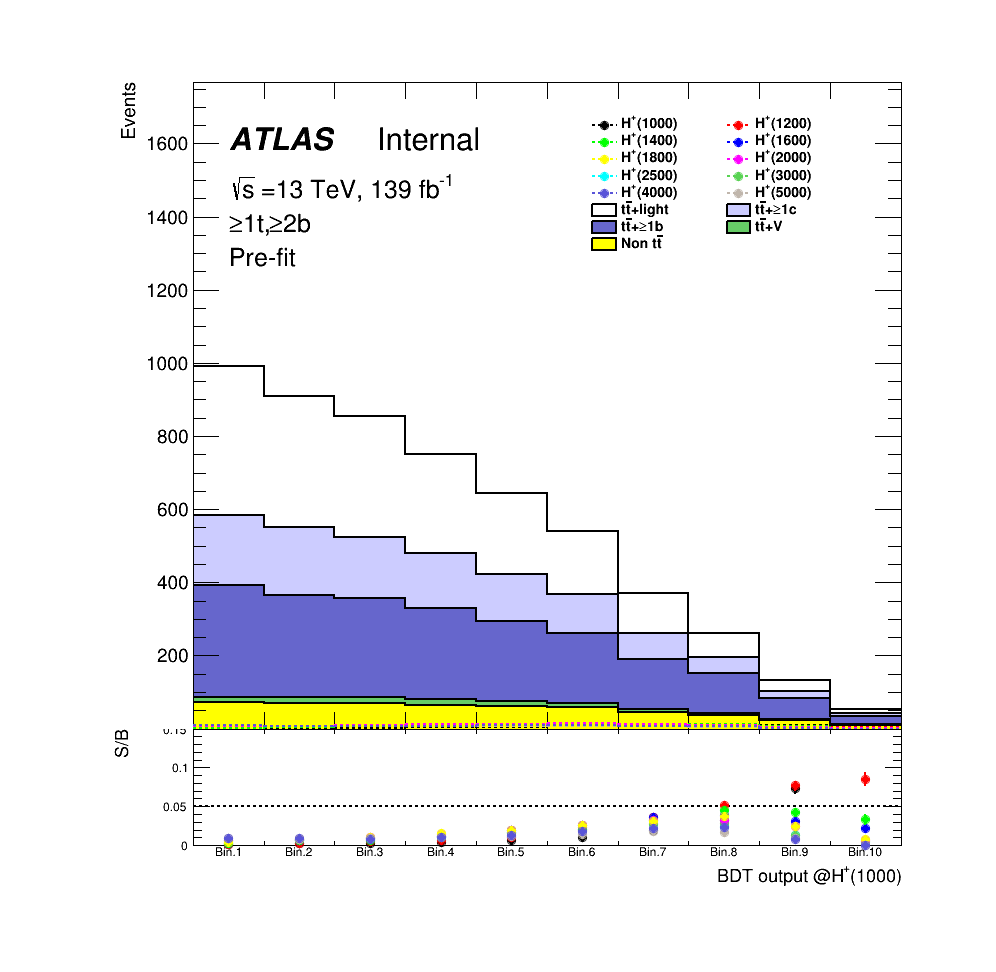
\includegraphics[width=0.30\textwidth]{images/SigBkgComparison/SOVERB_bdt_Hp1000_geq1tgeq2b.png}
    \label{fig:SOVERB_bdt_Hp1000_geq1tgeq2b}
  }
  \subfloat[] {
    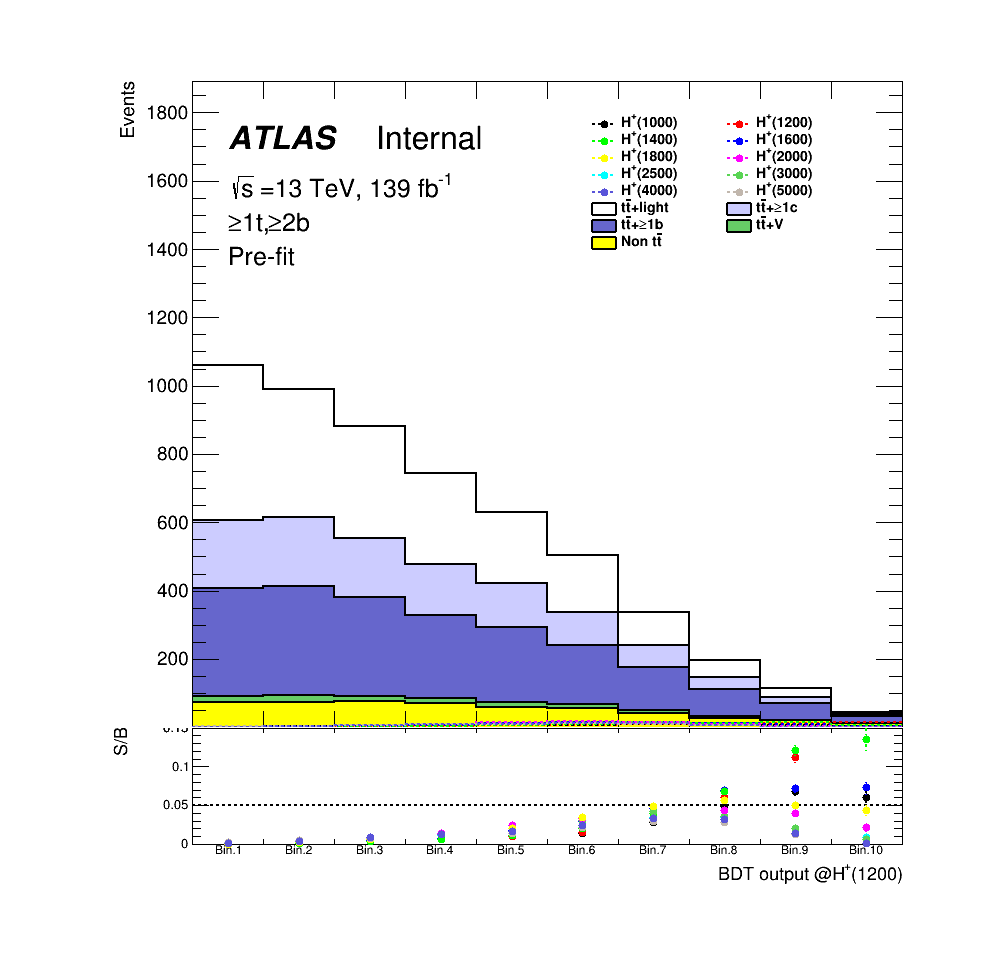
\includegraphics[width=0.30\textwidth]{images/SigBkgComparison/SOVERB_bdt_Hp1200_geq1tgeq2b.png}
    \label{fig:SOVERB_bdt_Hp1200_geq1tgeq2b}
  }
  \subfloat[] {
    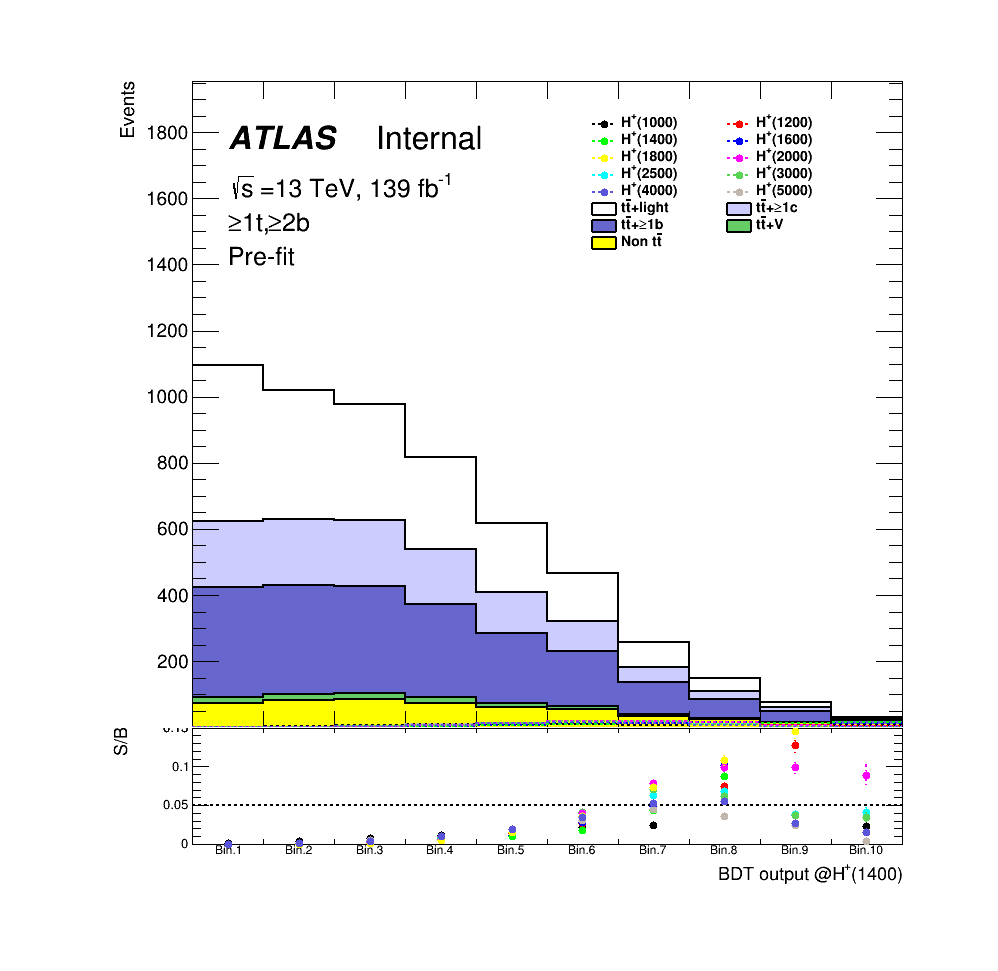
\includegraphics[width=0.30\textwidth]{images/SigBkgComparison/SOVERB_bdt_Hp1400_geq1tgeq2b.png}
    \label{fig:SOVERB_bdt_Hp1400_geq1tgeq2b}
  }\\
  \subfloat[] {
    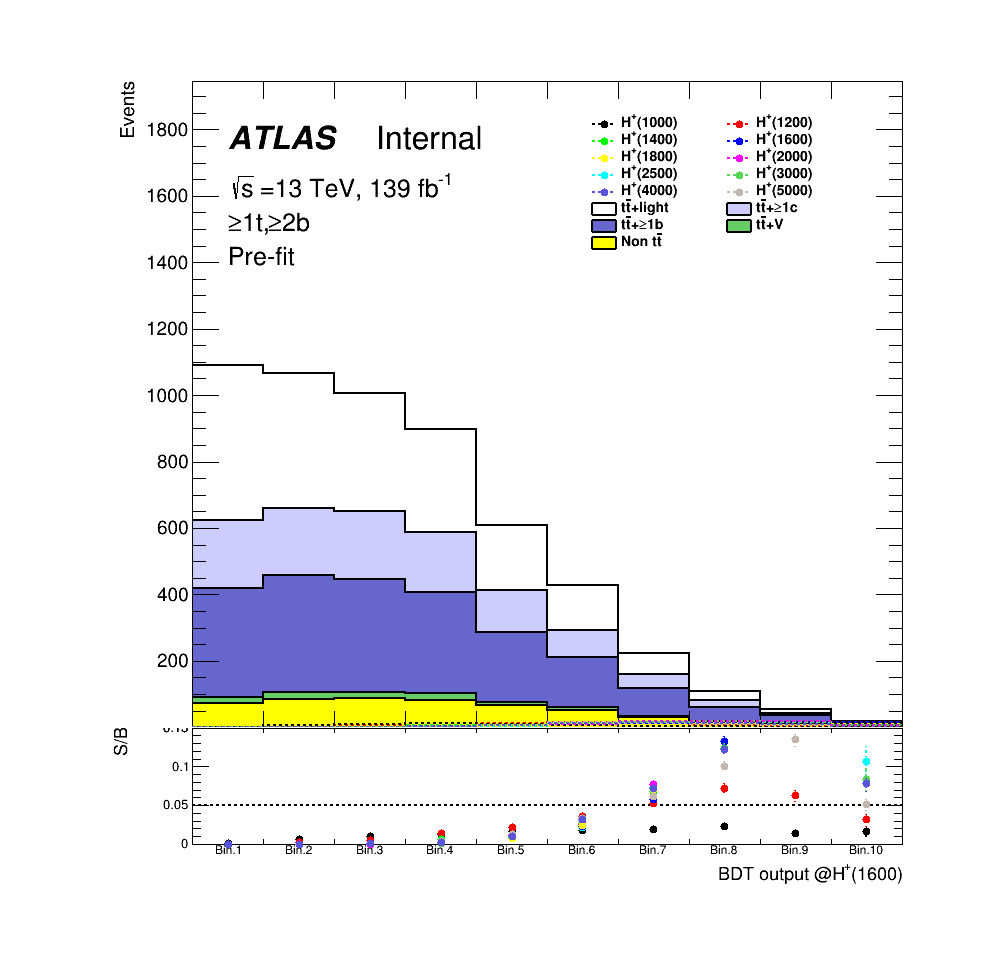
\includegraphics[width=0.30\textwidth]{images/SigBkgComparison/SOVERB_bdt_Hp1600_geq1tgeq2b.png}
    \label{fig:SOVERB_bdt_Hp1600_geq1tgeq2b}
  }
  \subfloat[] {
    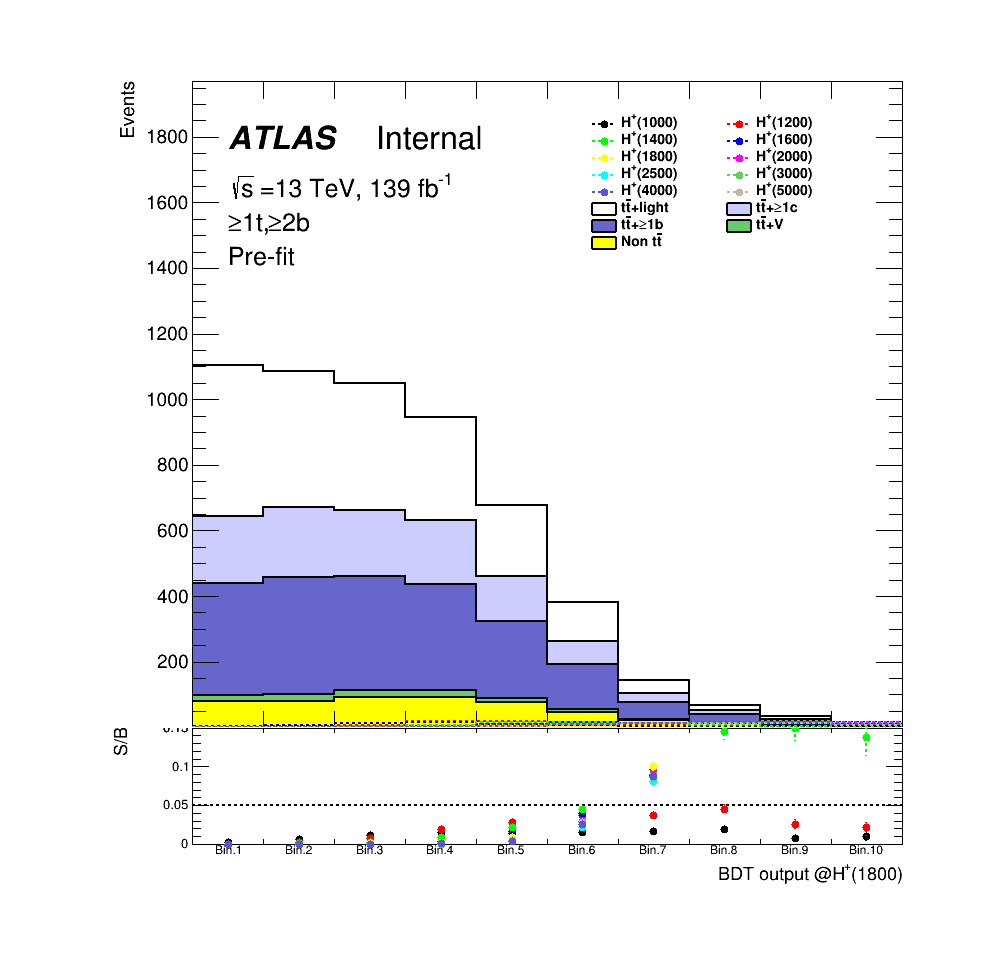
\includegraphics[width=0.30\textwidth]{images/SigBkgComparison/SOVERB_bdt_Hp1800_geq1tgeq2b.png}
    \label{fig:SOVERB_bdt_Hp1800_geq1tgeq2b}
  }
  \subfloat[] {
    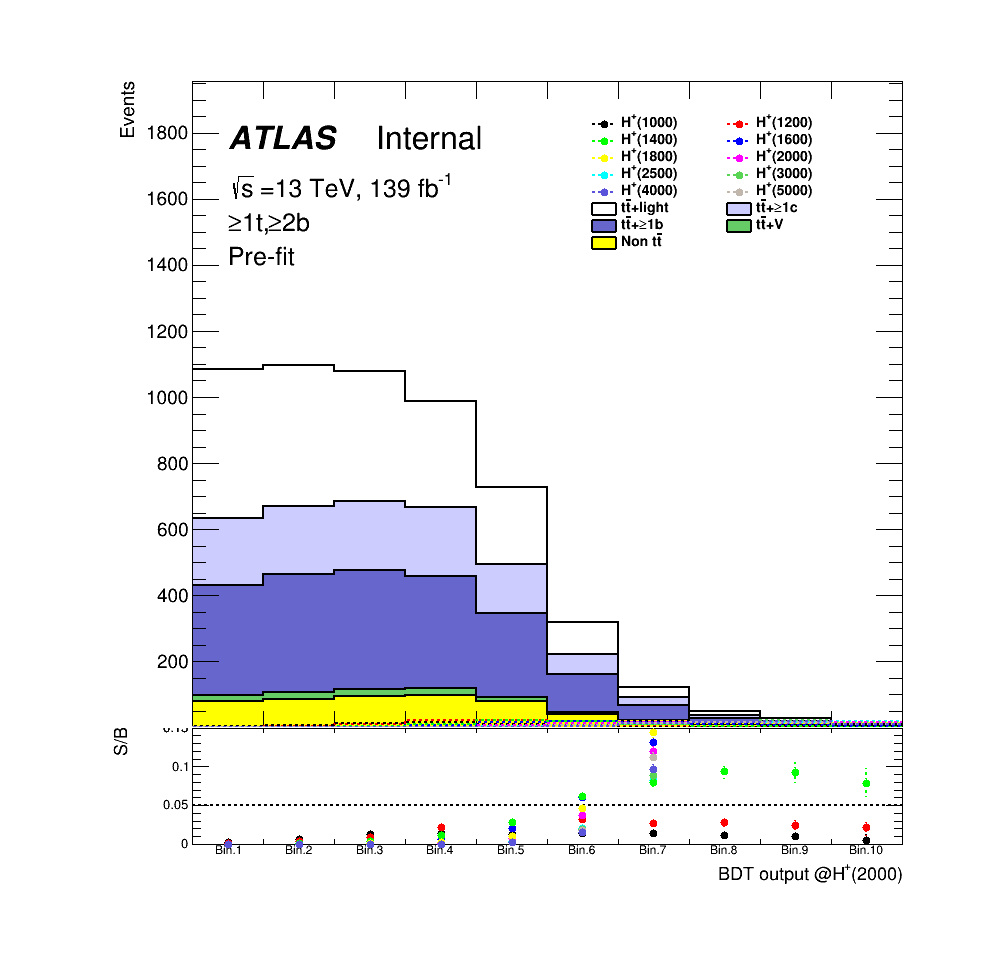
\includegraphics[width=0.30\textwidth]{images/SigBkgComparison/SOVERB_bdt_Hp2000_geq1tgeq2b.png}
    \label{fig:SOVERB_bdt_Hp2000_geq1tgeq2b}
  }\\
  \subfloat[] {
    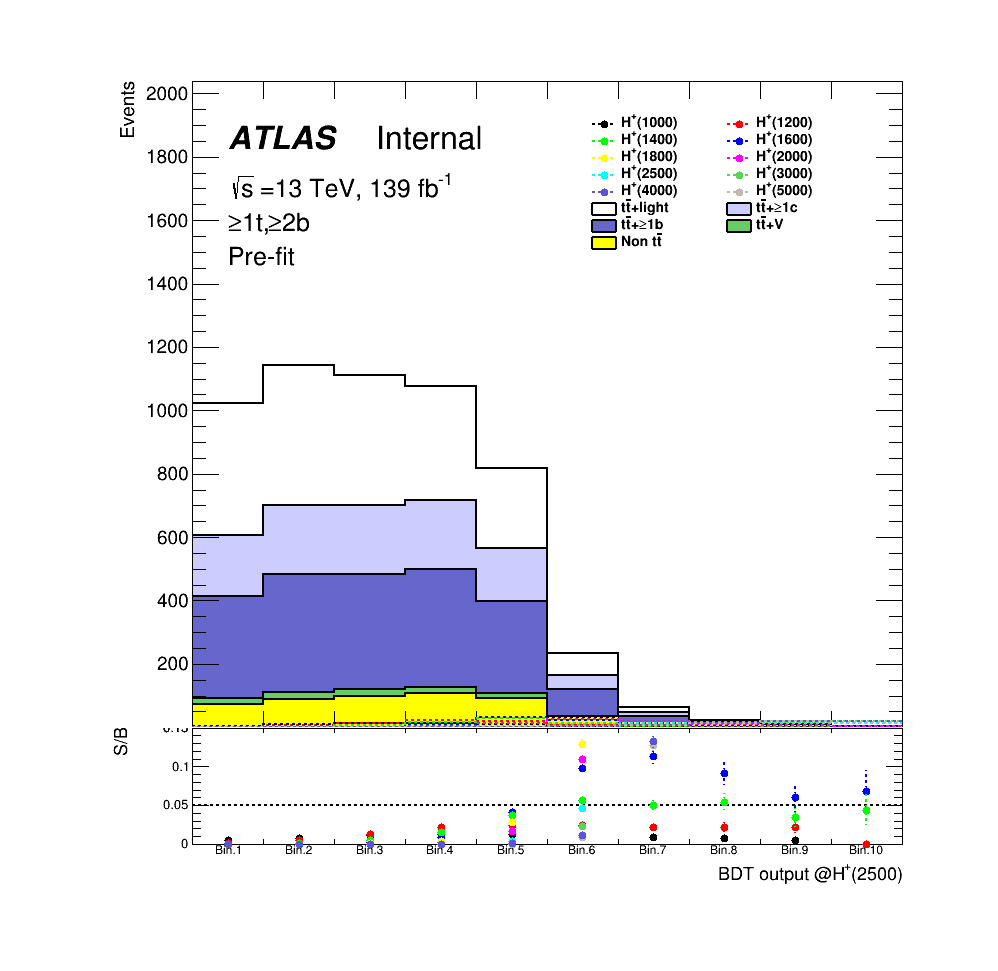
\includegraphics[width=0.30\textwidth]{images/SigBkgComparison/SOVERB_bdt_Hp2500_geq1tgeq2b.png}
    \label{fig:SOVERB_bdt_Hp2500_geq1tgeq2b}
  }
  \subfloat[] {
    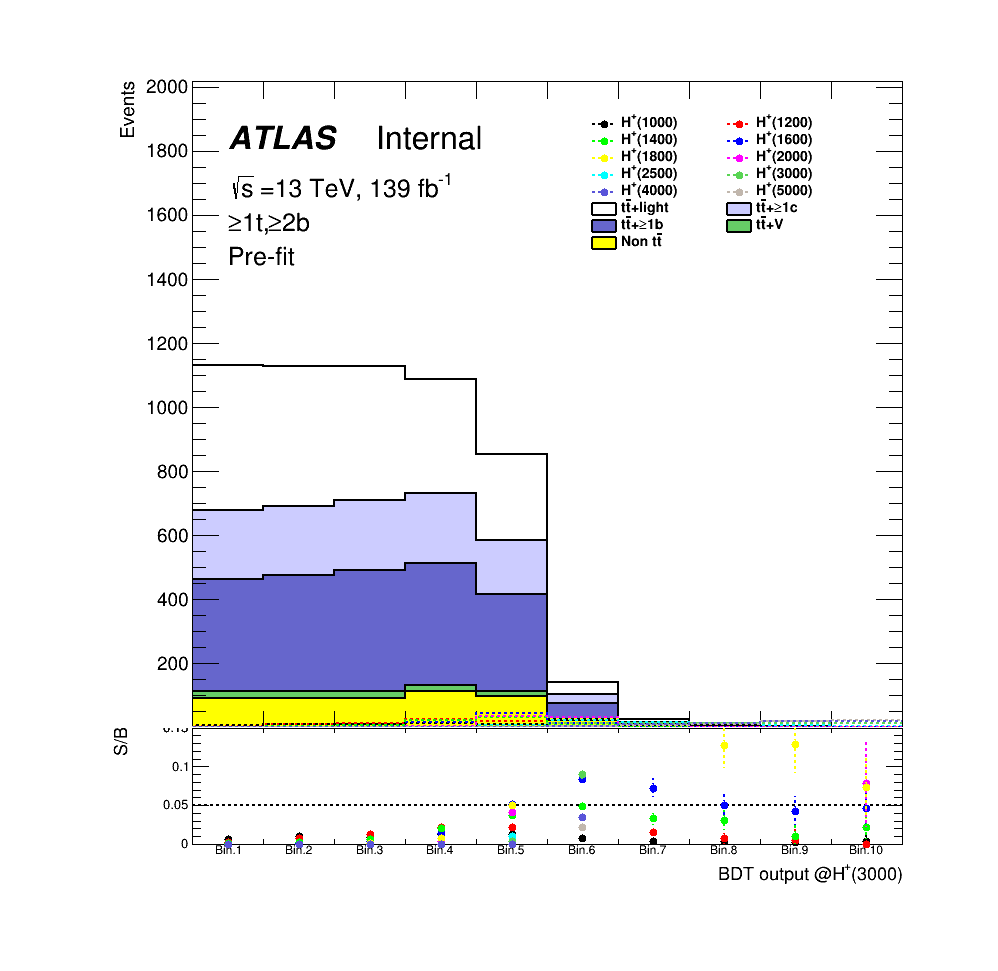
\includegraphics[width=0.30\textwidth]{images/SigBkgComparison/SOVERB_bdt_Hp3000_geq1tgeq2b.png}
    \label{fig:SOVERB_bdt_Hp3000_geq1tgeq2b}
  }
  \subfloat[] {
    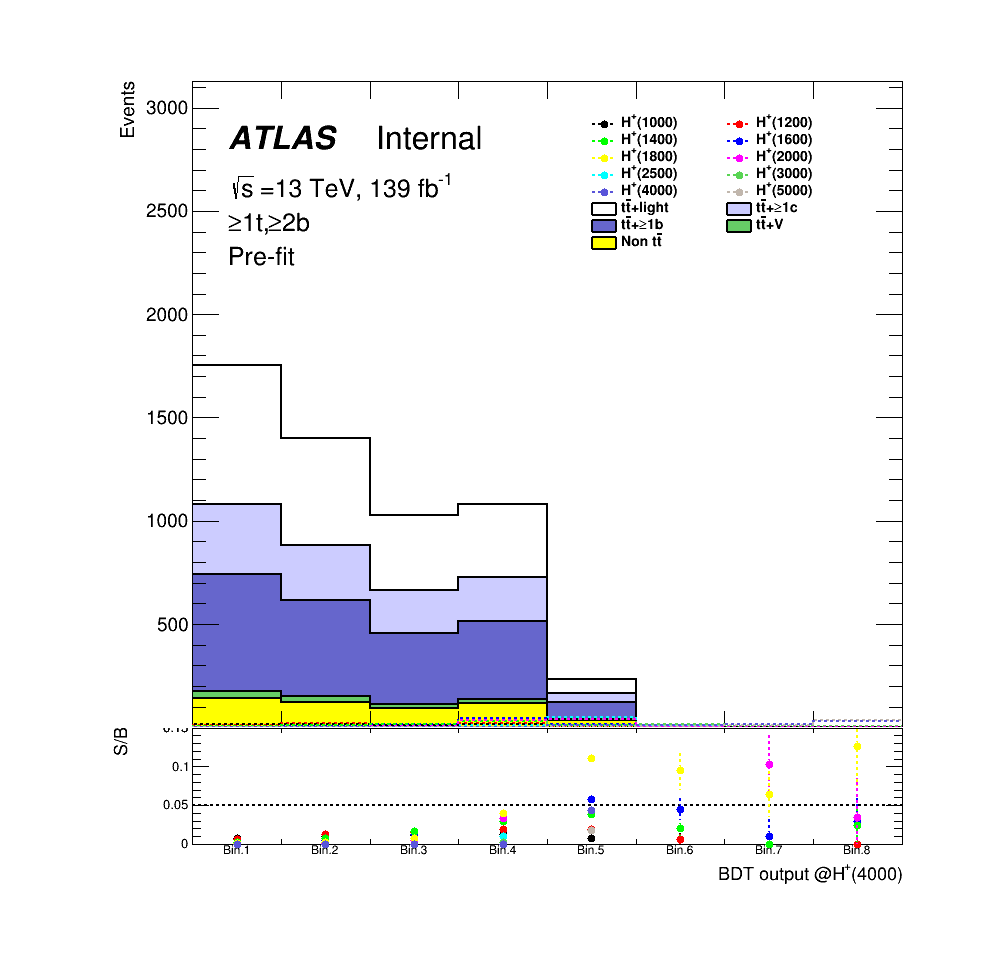
\includegraphics[width=0.30\textwidth]{images/SigBkgComparison/SOVERB_bdt_Hp4000_geq1tgeq2b.png}
    \label{fig:SOVERB_bdt_Hp4000_geq1tgeq2b}
  }\\
  \subfloat[] {
    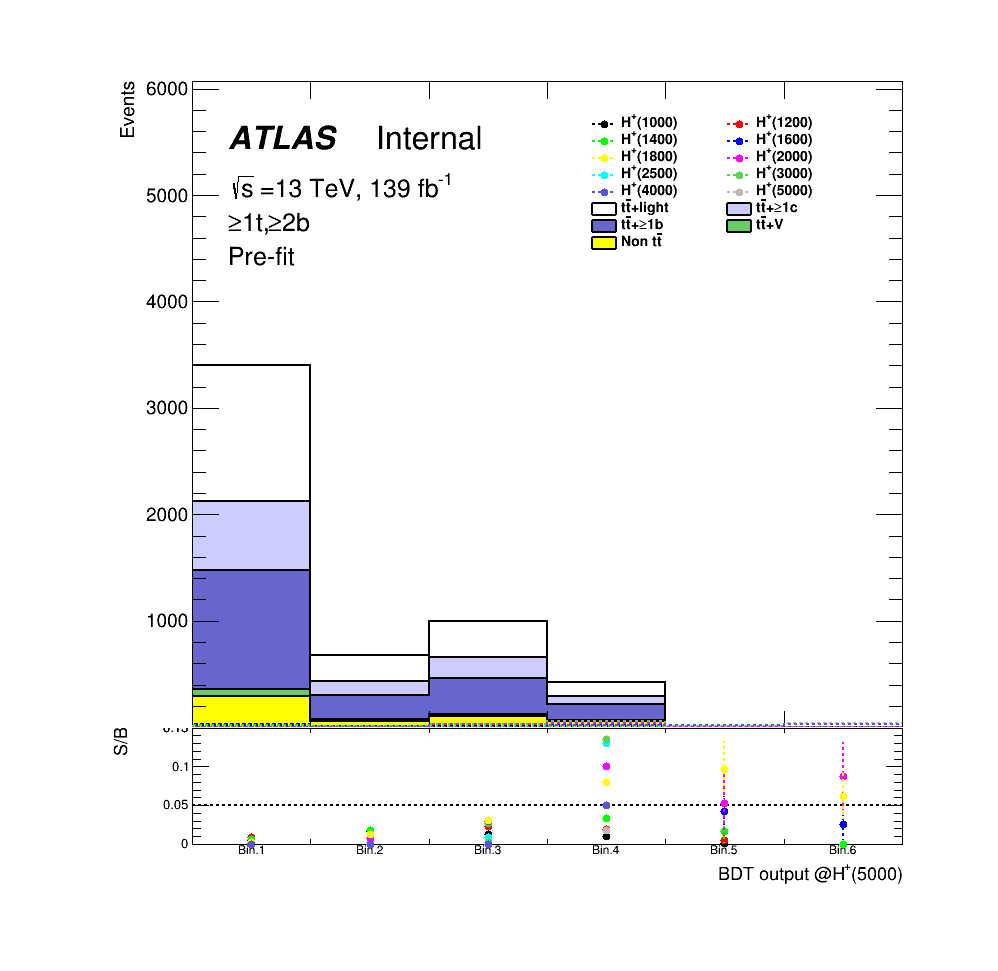
\includegraphics[width=0.30\textwidth]{images/SigBkgComparison/SOVERB_bdt_Hp5000_geq1tgeq2b.png}
    \label{fig:SOVERB_bdt_Hp5000_geq1tgeq2b}
  }
\end{figure}  